\documentclass[a4paper]{article}

%Tutti gli usepackage vanno qui

\usepackage{geometry}
\usepackage[italian]{babel}
\usepackage[utf8]{inputenc}
\usepackage[T1]{fontenc}
\usepackage{tabularx}
\usepackage{longtable}
\usepackage{hyperref}
\usepackage{enumitem}
\hypersetup{
	colorlinks=true,
	linkcolor=black,
	filecolor=magenta,      
	urlcolor=blue,
}
% Numerazione figure 
\let\counterwithout\relax
\let\counterwithin\relax
\usepackage{chngcntr}

\counterwithin{table}{subsection}
\counterwithin{figure}{subsection}

\usepackage[bottom]{footmisc}
\usepackage{fancyhdr}
\usepackage{titlesec}
\setcounter{secnumdepth}{4}
\usepackage{amsmath, amssymb}
\usepackage{array}
\usepackage{graphicx}

%\usepackage{float}
\usepackage{layouts}
\usepackage{float}
\usepackage{eurosym}


\usepackage{layouts}
\usepackage{float}
\usepackage{eurosym}

%Comandi di impaginazione uguale per tutti i documenti
\pagestyle{fancy}
\lhead{
\includegraphics[scale=0.07]{res/images/logo8_crop.png}}
%Titolo del documento
\rhead{\doctitle{}}
\rfoot{\thepage}
\cfoot{}
\setlength{\headheight}{35pt}
\setcounter{tocdepth}{4}
\setcounter{secnumdepth}{4}
\renewcommand{\footrulewidth}{0.4pt}

% multirow per tabelle
\usepackage{multirow}

% Permette tabelle su più pagine

%\usepackage{longtable}


% colore di sfondo per le celle
\usepackage[table]{xcolor}

%COMANDI TABELLE
\newcommand{\rowcolorhead}{\rowcolor[HTML]{56A5EC}} %intestazione 
\newcommand{\rowcolorlight}{\rowcolor[HTML]{fafafa}} %righe chiare/dispari
\newcommand{\rowcolordark}{\rowcolor[HTML]{e1f5fe}} %righe scure/pari
\newcommand{\colorhead}{\color[HTML]{FFFFFF}} %testo intestazione
\newcommand{\colorbody}{\color[HTML]{000000}} %testo righe
\newcommand{\tabitem}{~~\rlap{\textbullet}~~}

\newcommand{\glo}{$_{G}$}
\newcommand{\glosp}{$_{G}$ }

\definecolor{pari}{HTML}{E1F5
\definecolor{dispari}{HTML}{FAFAFA}


%Lista dei comandi personalizzati
\newcommand{\doctitle}{Verbale interno 2019-02-20}
\newcommand{\rev}{1.0.0}
\newcommand{\approv}{}
\newcommand{\ver}{}
\newcommand{\red}{Matteo Santinon}
\newcommand{\stato}{Approvato}
\newcommand{\uso}{Interno}
\newcommand{\describedoc}{Riassunto dell'incontro del gruppo \textit{8Lab 
Solutions} tenutosi il 2019-02-20.}
\newcommand{\destinatari}{8Lab Solutions\\& Prof. Tullio Vardanega\\& Prof. Riccardo Cardin}




\makeindex

\begin{document}

\thispagestyle{empty}
\begin{titlepage}
	\begin{center}
		
\includegraphics[scale = 0.3]{res/images/logo8_crop.png}\\
		\large \textbf{8Lab Solutions - Progetto "Soldino"} \\
		\vfill
		\Huge \textbf{\doctitle}
		\vspace*{\fill}
        
        \vfill
        \large
        \begin{tabular}{r|l}
                        \textbf{Versione} & \rev{} \\
                        \textbf{Approvazione} & \approv{} \\
                        \textbf{Redazione} & \red{} \\
                        \textbf{Verifica} & \ver{} \\
                        \textbf{Stato} & \stato{} \\
                        \textbf{Uso} & \uso{} \\
                        \textbf{Destinato a} & \parbox[t]{5cm}{8Lab Solutions
                        \\Prof. Tullio Vardanega\\Prof. Riccardo Cardin}
                \end{tabular}
                \vfill
                \normalsize
                \textbf{Descrizione}\\
                \describedoc
                \vfill
                \small
                \texttt{8labsolutions@gmail.com}
	\end{center}
\end{titlepage}


\pagebreak
\section*{Changelog}
\renewcommand{\arraystretch}{1.5}
\rowcolors{2}{pari}{dispari}
	\begin{longtable}{ 
			>{\centering}p{0.09\textwidth} 
			>{\centering}p{0.13\textwidth}
			>{\centering}p{0.2\textwidth} 
			>{\centering}p{0.16\textwidth} 
			>{}p{0.2775\textwidth} }
		
		\rowcolorhead
		\textbf{\color{white}Version} & 
		\textbf{\color{white}Date} & 
		\textbf{\color{white}Name} & 
		\textbf{\color{white}Role} &
		\centering \textbf{\color{white}Description} 
		\tabularnewline  
		\endfirsthead
		\rowcolorhead
		\textbf{\color{white}Version} & 
		\textbf{\color{white}Date} & 
		\textbf{\color{white}Name} & 
		\textbf{\color{white}Role} &
		\centering \textbf{\color{white}Description} 
		\tabularnewline  
		\endhead
		
		1.0.0 & 2019-03-30 & PLACEHOLDER & \textbf{Project Manager} &
		Approval
		\tabularnewline
		
		0.2.0 & 2019-03-27 & PLACEHOLDER & \textbf{Verifier} &
		Verification
		\tabularnewline
		
		0.1.2 & 2019-03-25 & PLACEHOLDER & \textbf{RUOLO} &
		Written §5.3, §5.4 and §6
		\tabularnewline
		
		0.1.2 & 2019-03-25 & PLACEHOLDER & \textbf{RUOLO} &
		Written §4.4 and §4.5
		\tabularnewline
		
		0.1.1 & 2019-03-24 & PLACEHOLDER & \textbf{RUOLO} &
		Written §3.3 and §4.3
		\tabularnewline
		
		0.1.0 & 2019-03-22 & PLACEHOLDER & \textbf{Verifier} &
		Verification
		\tabularnewline
		
		0.0.4 & 2019-03-21 & PLACEHOLDER & \textbf{RUOLO} &
		Written §3.2, §4.2 and §5.2
		\tabularnewline
		
		0.0.3 & 2019-03-21 & PLACEHOLDER & \textbf{RUOLO} &
		Written §3.1, §4.1 and §5.1
		\tabularnewline
		
		0.0.2 & 2019-03-20 & PLACEHOLDER & \textbf{RUOLO} &
		Written §1 and §2
		\tabularnewline
		
		0.0.1 & 2019-03-20 & Federico Bicciato & 
		\textbf{RUOLO} & Created document's structure.
		\tabularnewline
		
	
	\end{longtable}
\renewcommand{\arraystretch}{1} 


\counterwithin{table}{subsection}
\counterwithin{figure}{subsection}

\pagebreak

\tableofcontents

\pagebreak

\listoffigures

\pagebreak

\listoftables

\pagebreak

\counterwithin{table}{subsection}
\counterwithin{figure}{subsection}
\section{Introduzione}
\subsection{Scopo del documento}
Questo documento ha lo scopo di definire delle regole di base che tutti i membri 
di \textit{8Lab Solutions} devono rispettare nello svolgimento del progetto, 
così da garantire uniformità in tutto il materiale. Verrà utilizzato un 
approccio incrementale, volto a normare passo passo ogni decisione discussa e 
concordata tra tutti i membri del gruppo. Ciascun componente è obbligato a 
prendere visione di tale documento e a rispettare le norme in esso descritte 
allo scopo di perseguire la coesione\glosp all'interno del team.

\subsection{Scopo del prodotto}
Il capitolato\glosp C6 ha per obiettivo lo sviluppo di una piattaforma chiamata \textit{Soldino} che è basata sull'infrastruttura Ethereum\glo{} e funzionante tramite il meccanismo degli smart contracts\glo{}. \textit{Soldino} è gestita dal governo\glosp e ha lo scopo di assistere le aziende nella gestione dell'IVA riguardo tutte le operazioni di compravendita di beni e servizi. Il governo può coniare e 
distribuire la moneta utilizzata in queste transazioni, mentre i cittadini 
potranno acquistare i beni utilizzando tale valuta. La piattaforma, dunque, 
intende divenire un punto di incontro tra governo, aziende e cittadini.

\subsection{Glossario}
Al fine di evitare possibili ambiguità relative al linguaggio utilizzato nei documenti formali, viene fornito il \textit{Glossario v2.0.0}. In questo documento vengono definiti e descritti tutti i termini con un significato particolare. Per facilitare la lettura, i termini saranno contrassegnati da una 'G' a pedice.

\subsection{Riferimenti}
\subsubsection{Riferimenti normativi}
\begin{itemize}

	\item \textbf{Capitolato d'appalto C6 - Soldino, piattaforma Ethereum per pagamenti IVA}: \\
		\url{https://www.math.unipd.it/~tullio/IS-1/2018/Progetto/C6.pdf};
%verbali normativi PLACEHOLDER
\end{itemize}

\subsubsection{Riferimenti informativi}
\begin{itemize}
	\item \textbf{ Standard ISO/IEC 12207:1995}:\\* 
	\url{https://www.math.unipd.it/~tullio/IS-1/2009/Approfondimenti/ISO_12207-1995.pdf};
	\item \textbf{La qualità secondo ISO/IEC 9126}: \\*
	\url{http://www.colonese.it/00-Manuali_Pubblicatii/07-ISO-IEC9126_v2.pdf};
	\item \textbf{Slide L05 del corso Ingegneria del Software - Ciclo di vita 
	del software}:\\
		\url{https://www.math.unipd.it/~tullio/IS-1/2016/Dispense/L05.pdf};
	\item \textbf{Guide to the Software Engineering Body of Knowledge(SWEBOK), 2004} \\*
		\url{http://www.math.unipd.it/~	tullio/IS-1/2007/Approfondimenti/SWEBOK.pdf};
	\item \textbf{Software Engineering - Ian Sommerville - 9 th Edition (2010)}: \\*
		(formato cartaceo);
	\item \textbf{Documentazione git}: \\*
		\url{https://www.atlassian.com/git};
	\item \textbf{Standard ISO 8601}: \\*
		\url{https://it.wikipedia.org/wiki/ISO_8601}
	\item \textbf{Snake Case}\glo: \\*
		\url{https://it.wikipedia.org/wiki/Snake_case}
	\item \textbf{Airbnb JavaScript style guide}: \\*
		\url{https://github.com/airbnb/javascript/blob/master/README.md}
	
	
	
	
\end{itemize}

\pagebreak
\section{Qualità di processo}
Per ricercare qualità nello svolgimento del progetto si adoperano dei processi. Inizialmente, tali processi sono stati scelti tra quelli proposti nello standard ISO/IEC/IEEE 12207:2017; successivamente sono stati semplificati.\newline 
Il risultato sono i processi esposti a seguito.

%\subsection{Processo di Costruzione del Software}. Opzione per il futuro.

\subsection{Processi Tecnici}
	\subsubsection{Processo di Analisi dei Requisiti}
	Mediante il processo le informazioni ottenute dalle varie fonti sono trasformate in forma di casi d'uso e requisiti.
	Questa forma fornisce una descrizione dettagliata del sistema e definisce il funzionamento e le caratteristiche di ogni sua parte.
		\paragraph{Obiettivi}
		\begin{itemize}
			\item formulare la definizione di casi d'uso e requisiti;
			\item ottenere la loro approvazione;
			\item tracciare il loro cambiamento nel tempo.
		\end{itemize}		
		\paragraph{Strategia}
		\begin{itemize}
			\item considerare lo scopo del progetto e le richieste degli stakeholder;
			\item esprimere ciò in forma di requisiti, classificati in obbligatori, desiderabili e opzionali;
			\item valutare il corpo dei requisiti e negoziare cambiamenti se necessario;
			\item ottenere la loro approvazione da parte del proponente;
		\end{itemize}
		Disporre del tracciamento dei requisiti del sistema.
		\paragraph{Metriche}
			\subparagraph{Percentuale di requisiti obbligatori soddisfatti - PROS} Indica appunto la percentuale di requisiti obbligatori soddisfatti.
			\begin{itemize}
				\item misurazione: valore percentuale: $ PROS = \frac{requisiti\ obbligatori\ soddisfatti}{requisiti\ obbligatori\ totali}$;
				\item valore preferibile: $100\%$;
				\item valore accettabile: $100\%$.
			\end{itemize}
		
	\subsubsection{Processo di Definizione dell'Architettura}
	Tradurre i requisiti in un modello architetturale del sistema.
	Il modello è ad alto livello di dettaglio: in esso il sistema è costituito da macro-componenti, utili a capire il funzionamento delle parti, ma non ancora realizzabili nella pratica.\newline
	Nel processo vanno considerati in particolare il tipo di software da produrre, le caratteristiche desiderate e i suoi requisiti non funzionali per scegliere l'architettura più adatta.
		\paragraph{Obiettivi}
		\begin{itemize}
			\item agevolare la realizzazione fornendo un'architettura adeguata;
			\item perseguire la correttezza per costruzione;
			\item comprendere meglio il sistema scomponendolo in parti;
			\item progettare adoperando stili architetturali e design pattern.
		\end{itemize}
		\paragraph{Strategia}
		\begin{itemize}
			\item valutare il tipo di software da produrre, le caratteristiche desiderate, i casi d'uso e i requisiti da soddisfare;
			\item valutare i modelli architetturali secondo il punto precedente e scegliere il più adeguato;
			\item individuare nel modello i macro-componenti del sistema;
			\item comprendere e definire le relazioni tra i componenti.
		\end{itemize}
		\paragraph{Metriche}
			\subparagraph{Structural Fan-in \textbf{SFIN}}
			Indica quante componenti utilizzano un dato modulo. Un alto valore indica un alto riuso della componente.
			\begin{itemize}
				\item \textbf{Misurazione}: valore intero: conteggio delle componenti;
				\item \textbf{Valore preferibile}: $ \geq 1$;
				\item \textbf{Valore accettabile}: $ \geq 0$.
			\end{itemize}
			\subparagraph{Structural Fan-out \textbf{SFOUT}}
			Indica quante componenti vengono utilizzate dalla componente in esame. Un alto valore indica un alto
accoppiamento della componente.
			\begin{itemize}
				\item \textbf{Misurazione}: valore intero: conteggio delle componenti;
				\item \textbf{Valore preferibile}: $ = 0$;
				\item \textbf{Valore accettabile}: $ \leq 6$.
			\end{itemize}
			
	\subsubsection{Processo di Progettazione di Design}
	\textit{Nota: in questo contesto si usano i termini componente, modulo e unità alternandoli. Lo stesso oggetto possiede le proprietà espresse dai tre termini (unitarietà, modularità e composizione), e a seconda del contesto si preferisce l'uno all'altro termine.}\newline 
	La Progettazione di Design segue la Definizione dell'Architettura e prevede la scomposizione delle macro-componenti in moduli più piccoli che sono:
	\begin{itemize}
		\item facilmente comprensibili;
		\item strettamente collegati ai requisiti funzionali;
		\item implementabili da un singolo programmatore.
	\end{itemize}
		\paragraph{Obiettivi}
		\begin{itemize}
			\item tradurre i requisiti in unità di codice, i moduli;
			\item favorire il lavoro dei programmatori con compiti individuali relativi ai singoli moduli;
			\item produrre un sistema software fatto di componenti ed utilizzabile;
			\item mantenere il tracciamento tra requisiti e componenti;
		\end{itemize}
		\paragraph{Strategia}
		\begin{itemize}
			\item scomporre le componenti architetturali in componenti piccole;
			\item implementare le componenti individuate;
		\end{itemize}
		\paragraph{Metriche}
			\subparagraph{Accoppiamento tra le classi di oggetti - CBO} 
			Una classe è accoppiata a una seconda se usa metodi o variabili definiti nella seconda. 
			\begin{itemize}
				\item misurazione: valore intero: $CBO$;
				\item valore preferibile: $0 \leq CBO \leq 1$;
				\item valore accettabile: $0 \leq CBO \leq 6$.
			\end{itemize}
		
\subsection{Processi di Gestione Tecnica}
	\subsubsection{Processo di Pianificazione di Progetto}
	Il processo consiste nella produzione di un Piano di Progetto e nella sua manutenzione. Il piano governa le risorse a disposizione, ovvero tempi, costi e ruoli.
		\paragraph{Obiettivi}
		\begin{itemize}
			\item avere a disposizione piani e obiettivi ben definiti;
			\item aver definito ruoli, responsabilità, obblighi e autorità a cui rispondere;
			\item aver allocato le risorse e i beni necessari;
			\item attivare il piano per sostenere il progetto.
		\end{itemize}	
		\paragraph{Strategia}
		\begin{itemize}
			\item produrre la pianificazione delle attività;
			\item mantenerla aggiornata mentre esse vengono svolte;
			\item usarla come riferimento e supporto.
		\end{itemize}		
		\paragraph{Metriche}
		\subparagraph{BAC: Budget at Completion}
		Budget totale allocato per il progetto
		\begin{itemize}
			\item misurazione: numero intero;
			% PLACEHOLDER: Aggiornare i 2 item qui sotto
			\item valore preferibile: $pari\ al\ preventivo$;
			\item valore accettabile: $di\ poco\ maggiore\ o\ pari\ al\ preventivo$.
		\end{itemize}
			\subparagraph{AC: Actual Cost}
			Il denaro speso fino al momento del calcolo.
			\begin{itemize}
				\item  misurazione: numero intero;
				\item  valore preferibile: $0 \leq AC < PV$;
				\item  valore accettabile: $0 \leq AC \leq budget\ totale\ $;
			\end{itemize}
			\subparagraph{EV - Earned Value}
			Metrica di utilità. Si tratta del valore del lavoro fatto fino al momento del calcolo; corrisponde al denaro guadagnato fino a quel momento.
			\begin{itemize}
				\item  misurazione: $BAC \cdot \%\ di\ lavoro\ completato\ $;
				\item  valore preferibile: $ \geq 0$;
				\item  valore accettabile: $ \geq 0$.
			\end{itemize}
			\subparagraph{PV: Planned Value}
			Si tratta del valore del lavoro pianificato al momento del calcolo: corrisponde al denaro che si dovrebbe aver guadagnato in quel momento.
			\begin{itemize}
				\item  misurazione: $BAC \cdot \%\ di\ lavoro\ pianificato\ $;
				\item  valore preferibile: $ \geq 0$;
				\item  valore accettabile: $ \geq 0$;
			\end{itemize}			
			\subparagraph{SV: Schedule Variance}
			Dice se si è avanti o indietro nello svolgimento del progetto rispetto alla pianificazione.
			\begin{itemize}
				\item misurazione: $SV = EV - PV$
				\item valore preferibile: $ > 0$;
				\item valore accettabile: 0;
			\end{itemize}
			\subparagraph{Cost Variance}
			Differenza tra il costo del lavoro effettivamente completato e quello pianificato. Una CV positiva indica che si sta rispettando il budget.
			\begin{itemize}
				\item misurazione: $CV = EV - AC$;
				\item valore preferibile: $ > 0$
				\item valore accettabile: $ \geq 0$
			\end{itemize}

	\subsubsection{Processo di Verifica}
	Il processo consiste nella ricerca e correzione di anomalie e difetti nei processi e prodotti del progetto, mediante tecniche predefinite e se possibile automatiche.
		\paragraph{Obiettivi}
		\begin{itemize}
			\item individuare e correggere le anomalie;
			\item provare che il sistema soddisfi i requisiti.
		\end{itemize}	
		\paragraph{Strategia}
		\begin{itemize}
			\item individuare tecniche e strumenti di verifica;
			\item applicarli;
			\item affinarli con l'esperienza;
		\end{itemize}	
		\paragraph{Metriche}
			\subparagraph{Code Coverage - CC}
				Indica il numero di righe di codice percorse dai test durante la loro esecuzione. Per linee di codice totali si intende tutte quelle appartenenti all'unità in fase di test.
				\begin{itemize}
					\item misurazione: valore percentuale: $CC = \frac{linee\ di\ codice\ percorse}{linee\ di\ codice\ totali}$;
					\item valore preferibile: $100\%$;
					\item valore accettabile: $75\%$.
				\end{itemize}
			% a grana più fine ci sarebbero: function coverage, loop coverage, branch coverage

	\subsubsection{Processo di Gestione dell'Informazione}
	Il processo consiste nella produzione di informazioni, la cui forma tipica è  documentale, e nella loro gestione. I documenti sono prodotti a supporto di tutte le attività di progetto.
		\paragraph{Obiettivi}
			Si costruisce la documentazione affinché sia un body of knowledge % PLACEHOLDER: glossario
			che raccoglie la conoscenza in modo:
			\begin{itemize}
				\item completo;
				\item non ambiguo;
				\item modulare e fatto di parti coese;
				\item trasparente, adatto alla trasmissione delle informazioni;
				\item disponibile esternamente.
			\end{itemize}
		\paragraph{Strategia}
		I documenti sono:
		\begin{itemize}
			\item prodotti in concomitanza con tutte le attività di sviluppo;
			\item prodotti in modo collaborativo;
			\item supportati da un glossario;
			\item supportati da Norme di Progetto;
			\item prodotti con strumenti software adatti alla collaborazione e alla modularità in \LaTeX{};
			\item ospitati in una repository pubblica su Github;
		\end{itemize}
		\paragraph{Metriche}
			\subparagraph{Indice Gunning fog}
			Indice della leggibilità del testo. Stima gli anni di educazione scolastica richiesti per comprendere il testo a una prima lettura.\newline
			Ha dei limiti: uno di questi è la sua definizione di \textit{parola complessa}, intesa come una parola di tre o più sillabe eccetto alcuni suffissi comuni.
			\begin{itemize}
				\item misurazione: valore intero: $ I_{GF} = 0.4 \cdot
				(
				\frac{numero\ di\ parole}{numero\ di\  frasi}
				+ 100 \cdot
				\frac{numero\ di\ parole\ complesse}{numero\ di\  frasi}
				) $;
				\item valore preferibile: $ \leq 12$;
				\item valore accettabile: $ \leq 16$.
			\end{itemize}
			\subparagraph{Indice di Gulpease}
			Indice della leggibilità del testo. Valuta la lunghezza delle parole e delle frasi rispetto al numero totale di lettere. 
			\begin{itemize}
				\item misurazione: valore intero da 0 a 100:\newline 	
				$I_G = 89+ \frac{(300 \cdot numero\ di\ frasi - 10 \cdot numero\ di\ lettere)}{numero\ di\ parole}$	
				\item valore preferibile: $80 < I_G < 100$;
				\item valore accettabile: $40 < I_G < 100$	
			\end{itemize}
			\subparagraph{Correttezza ortografica}
			Tutti i documenti non devono assolutamente contenere errori grammaticali o errori ortografici. 
			\begin{itemize}
				\item misurazione: valore intero: numero di errori grammaticali o ortografici per documento;
				\item Valore preferibile: 0;
				\item Valore accettabile: 0.
			\end{itemize}
			
\subsection{Processi Organizzativi}
	\subsubsection{Processo di Gestione della Qualità}
	Tale processo ha per scopo il raggiungimento di un grado soddisfacente di qualità nel progetto. Fornisce:
	\begin{itemize}
		\item obiettivi da perseguire;
		\item strumenti tecnici, come procedure e metriche.
	\end{itemize}
		\paragraph{Obiettivi}
		Garantire che i prodotti e processi rispettino gli standard di qualità richiesti.
		\paragraph{Strategia}
		\begin{itemize}
			\item pianificare le proprie azioni perseguendo gli obiettivi;
			\item utilizzare gli strumenti forniti per misurare e monitorare i risultati;
			\item reagire ai risultati aggiornando obiettivi, strategia e strumenti.
		\end{itemize}
		\paragraph{Metriche}
			\subparagraph{Percentuale di metriche soddisfatte - PMS}
			La percentuale di metriche soddisfatte valuta quante metriche raggiungono soglie accettabili sul numero totale delle metriche calcolate. Una bassa percentuale di soddisfazione può indicare poca qualità, metriche inadeguate o mancata correttezza nel calcolo.
			\begin{itemize}
				\item misurazione: $\frac{numero\ di\ metriche\ soddisfatte}{numero\ di\ metriche\ totali} $;
				\item valore preferibile: $ \geq 80\%$;
				\item valore accettabile: $ \geq 60\%$;
			\end{itemize}
		
\pagebreak
\section{Qualità di prodotto}
Per valutare la qualità del prodotto il gruppo ha deciso di far riferimento allo standard ISO/IEC 9126\glosp{} che definisce le caratteristiche di cui tener conto per produrre un prodotto di buona qualità. Le caratteristiche sono descritte attraverso dei parametri, che ne quantificano il grado di raggiungimento. Di seguito vengono citate le voci che il gruppo ha ritenuto rilevanti nel contesto del progetto.
	\subsection{Funzionalità}
	Capacità del prodotto di fornire funzioni che riescano a soddisfare tutti i requisiti, sia espliciti che impliciti, presenti nell'Analisi dei Requisiti.
		\subsubsection{Obiettivi}
		\begin{itemize}
			\item \textbf{Appropriatezza}: il prodotto deve mettere a disposizione un insieme di funzioni conformi agli obiettivi richiesti;
			\item \textbf{Accuratezza}: il prodotto deve fornire risultati attesti con il grado di precisione richiesto;
			\item \textbf{Conformità}: il prodotto deve aderire a determinati standard. %PLACEHOLDER è forse troppo ovvio?
		\end{itemize}
		\subsubsection{Metriche}
			\paragraph{Completezza dell'implementazione}
			La completezza del prodotto e il rispetto dei requisiti viene indicato da una percentuale.
			\begin{itemize}
			\item misurazione: si calcola con la seguente formula: \\
			\centerline { C = (1 - \(\frac{N\textsubscript{FNI}}{N\textsubscript{FI}} \))$ \cdot  100$ } \\
			dove N\textsubscript{FNI} indica il numero di funzionalità non implementate e N\textsubscript{FI} indica il numero di funzionalità individuate dall'analisi;
			\item valore preferibile: 100\%;
			\item valore accettabile: 100\%.
			\end{itemize}
	\subsection{Affidabilità}
	Capacità del prodotto di mantenere prestazioni elevate anche in caso di situazioni anomale o critiche.
		\subsubsection{Obiettivi}
		\begin{itemize}
			\item maturità: il prodotto deve evitare che si verifichino errori e malfunzionamenti;
			\item tolleranza agli errori: il prodotto mantiene alte prestazioni anche in caso di malfunzionamenti o di un uso scorretto.
		\end{itemize}
		\subsubsection{Metriche}
			\paragraph{Densità errori}
			L'abilità del prodotto di resistere a malfunzionamenti viene indicata con una percentuale.
			\begin{itemize}
			\item misurazione: si calcola con la seguente formula: \\
			\centerline{ M =  \(\frac{N\textsubscript{ER}}{N\textsubscript{TE}} \)$ \cdot 100$ }
			dove N\textsubscript{ER} indica il numero di errori rilevati durante il testing e N\textsubscript{TE} indica il numero di test eseguiti;
			\item valore preferibile: 0\%;
			\item valore accettabile: $\leq$ 10\%.
			\end{itemize}
	\subsection{Usabilità}
	Capacità del prodotto di essere di facile comprensione e utilizzo da parte degli utenti.
		\subsubsection{Obiettivi}
		\begin{itemize}
			\item comprensibilità: l'utente deve essere in grado di comprendere le funzionalità offerte dal prodotto e ad utilizzarle;
			\item apprendibilità: l'utente deve poter imparare facilmente ad utilizzare il prodotto;
			\item attrattività: il prodotto deve essere piacevole da usare.
		\end{itemize}
		\subsubsection{Metriche}
			\paragraph{Facilità di utilizzo}
			La facilità con cui l'utente raggiunge ciò che vuole viene rappresentata tramite il numero di click necessari per arrivare al contenuto desiderato.
			\begin{itemize}
			\item misurazione: click per raggiungere la schermata di checkout;
			\item valore preferibile: $\leq$ 10;
			\item valore accettabile: $\leq$ 15.
			\end{itemize}
			\paragraph{Facilità di apprendimento}
			La facilità con cui l'utente riesce ad imparare ad usare le funzionalità del prodotto viene rappresentata tramite il tempo medio che serve per comprenderle.
			\begin{itemize}
			\item misurazione: minuti per raggiungere pagina di checkout;
			\item valore preferibile: $\leq$ 3;
			\item valore accettabile: $\leq$ 5.
			\end{itemize}
			\paragraph{Profondità della gerarchia}
			La profondità del sito. Un sito per essere facile da utilizzare non deve essere troppo profondo.
			\begin{itemize}
			\item misurazione: livello di profondità della pagine;
			\item valore preferibile: $\leq$ 4;
			\item valore accettabile: $\leq$ 7.
			\end{itemize}
	\subsection{Manutenibilità}
	Capacità del prodotto di essere modificato, includendo correzioni, miglioramenti o adattamenti.
		\subsubsection{Obiettivi}
		\begin{itemize}
			\item analizzabilità: facilità con la quale è possibile analizzare il codice per localizzare un errore;
			\item modificabilità: capacità del prodotto di permettere l'implementazione di una modifica.
		\end{itemize}
		\subsubsection{Metriche}
			\paragraph{Facilità di comprensione}
			La facilità con cui è possibile comprendere cosa fa il codice può rappresentata dal numero di linee di commento nel codice.
			\begin{itemize}
			\item misurazione: Si può calcolare con la seguente formula: \\
			\centerline{R = \(\frac{N\textsubscript{LCOM}}{N\textsubscript{LCOD}} \) }
			dove N\textsubscript{LCOM} indica le linee di commento e N\textsubscript{LCOD} indica le linee di codice;
			\item valore preferibile: $\geq$ 0.20;
			\item valore accettabile: $\geq$ 0.10.
			\end{itemize}
			\paragraph{Semplicità delle funzioni}
			La facilità di un metodo può essere rappresentata dal numero di parametri per metodo: meno parametri ha una funzione più è semplice e intuitiva.
			\begin{itemize}
			\item misurazione: numero di parametri per metodo;
			\item valore preferibile $\leq$ 3;
			\item valore accettabile $\leq$ 6.
			\end{itemize}
			\paragraph{Semplicità delle classi}
			La facilità di una classe può essere rappresentata dal numero di metodi per classe: una classe con pochi metodi ha uno scopo ben preciso e facilmente comprensibile.
			\begin{itemize}
			\item misurazione: numero di metodi per classe;
			\item valore preferibile $\leq$ 8;
			\item valore accettabile $\leq$ 15.
			\end{itemize}
\pagebreak

\pagebreak
\section{Test}
I test sono attività che servono a verificare che il software prodotto implementi le funzionalità richieste.
\subsection{Test di accettazione} 
	\renewcommand{\arraystretch}{1.5}
	\rowcolors{2}{pari}{dispari}
	
	\begin{longtable}{ >{\centering}p{0.10\textwidth} >{}p{0.70\textwidth}
			>{\centering}p{0.10\textwidth} >{\centering}p{0.10\textwidth}}
			
		%\tabularnewline
		\caption{Riepilogo Test di Accettazione}\\	
		\rowcolorhead
		\textbf{\color{white}Codice} 
		& \centering\textbf{\color{white}Descrizione} 
		& \centering\textbf{\color{white}Stato}
		& \centering\textbf{\color{white}Esito} 
		\tabularnewline %\tabularnewline 
		\endfirsthead	
		
		\rowcolor{white}\caption[]{(continua)}\\	
		\rowcolorhead
		\textbf{\color{white}Codice} 
		& \centering\textbf{\centering\color{white}Descrizione} 
		& \centering\textbf{\color{white}Stato}
		& \centering\textbf{\color{white}Esito} 
		\tabularnewline %\tabularnewline 
		\endhead	
		
\hypertarget{TAFD1}{TAFD1} & L'utente deve poter accedere alla guida dell'applicazione. All'utente viene
		 chiesto di:
		 \begin{itemize}
		 	\item verificare che sia possibile accedere alla guida;
		 	\item verificare che la guida riporti informazioni riguardanti l'utilizzo di
		 	MetaMask\glo{};
		 	\item verificare che la guida riporti informazioni riguardanti il pagamento
		 	delle operazioni. 
		 \end{itemize} & \textit{NI} & \textit{NS}\\ \tabularnewline
\hypertarget{TAFO2}{TAFO2} & L'utente non ancora autenticato deve poter effettuare la registrazione al
		 sistema. All'utente viene chiesto di:
		 \begin{itemize}
		 	\item accedere alla pagina di registrazione;
		 	\item selezionare il tipo di utente;
		 	\item inserire i dati in base al tipo scelto.
		 \end{itemize} & \textit{NI} & \textit{NS}\\ \tabularnewline
\hypertarget{TAFO2.1}{TAFO2.1} & L'utente deve potersi registrare come cittadino. All'utente viene chiesto di:
		 \begin{itemize}
		 	\item accedere alla pagina di registrazione e scegliere la registrazione
		 	come cittadino;
		 	\item inserire l'email;
		 	\item inserire l'indirizzo;
		 	\item inserire il nome;
		 	\item inserire il cognome.
		 \end{itemize} & \textit{NI} & \textit{NS}\\ \tabularnewline
\hypertarget{TAFO2.2}{TAFO2.2} & L'utente deve potersi registrare come azienda. All'utente viene chiesto di:
		 \begin{itemize}
		 	\item accedere alla pagina di registrazione e scegliere la registrazione
		 	come azienda;
		 	\item inserire l'email;
		 	\item inserire la sede;
		 	\item inserire la partita IVA;
		 	\item inserire il nome.
		 \end{itemize} & \textit{NI} & \textit{NS}\\ \tabularnewline
\hypertarget{TAFO2.3}{TAFO2.3} & L'utente deve poter visualizzare un messaggio di errore nel caso in cui la
		 chiave reperita da MetaMask\glo{} durante la registrazione sia già presente
		 nel sistema. & \textit{NI} & \textit{NS}\\ \tabularnewline
\hypertarget{TAFO3.1}{TAFO3.1} & L'utente deve poter autenticarsi nel sistema in modo automatico attraverso
		 MetaMask\glo{}. All'utente è chiesto di:
		 \begin{itemize}
		 	\item accedere alla sezione per il login;
		 	\item verificare l'avvenuta autenticazione.
		 \end{itemize} & \textit{NI} & \textit{NS}\\ \tabularnewline
\hypertarget{TAFO4}{TAFO4} & L'utente deve potersi disconnettere dal sistema. All'utente viene chiesto di:
		 \begin{itemize}
		 	\item autenticarsi correttamente nel sistema;
		 	\item trovarsi in una qualsiasi delle pagine di navigazione destinate 
		 	all'utente;
		 	\item premere il tasto di logout;
		 	\item confermare di voler effettuare la disconnessione premendo il tasto 
		 	di conferma;
		 	\item verificare che la disconnessione sia avvenuta correttamente.
		 \end{itemize} & \textit{NI} & \textit{NS}\\ \tabularnewline
\hypertarget{TAFO5}{TAFO5} & L'utente autenticato come governo deve poter coniare Cubit\glo{}.
		 All'utente viene chiesto di:
		 \begin{itemize}
		 	\item autenticarsi correttamente nel sistema;
		 	\item trovarsi nella pagina per la coniazione della moneta;
		 	\item selezionare una quantità positiva di Cubit\glo{};
		 	\item dare conferma dell'operazione. 
		 \end{itemize} & \textit{NI} & \textit{NS}\\ \tabularnewline
\hypertarget{TAFO6}{TAFO6} & L'utente autenticato come governo deve poter distribuire Cubit\glo{}
		 agli utenti registrati come aziende o cittadini. All'utente viene chiesto di:
		 \begin{itemize}
		 	\item autenticarsi correttamente nel sistema;
		 	\item trovarsi nella pagina per la distribuzione della moneta;
		 	\item selezionare una quantità positiva di Cubit da 
		 	distribuire;
		 	\item selezionare la lista di utenti a cui trasferire i Cubit; 
		 	\item dare conferma dell'operazione. 
		 \end{itemize} & \textit{NI} & \textit{NS}\\ \tabularnewline
\hypertarget{TAFO8}{TAFO8} & L'utente autenticato come azienda o cittadino deve poter visualizzare i
		 prodotti in vendita nel sito. All'utente viene chiesto di:
		 \begin{itemize}
		 	\item accedere alla pagina dei prodotti in vendita nel sito;
		 	\item verificare che sia visualizzato il nome del prodotto;
		 	\item verificare che sia visualizzato il prezzo lordo\glo{} del prodotto;
		 	\item verificare che sia visualizzata la descrizione del prodotto;
		 	\item verificare che sia visualizzata la quantità relativa ad un certo
		 	prodotto in vendita nel sito;
		 	\item verificare che sia possibile cambiare la quantità selezionata relativa ad un prodotto in
		 	vendita nel sito.
		 \end{itemize} & \textit{NI} & \textit{NS}\\ \tabularnewline
\hypertarget{TAFO9}{TAFO9} & L'utente autenticato come azienda o cittadino deve poter aggiungere
		 al proprio carrello prodotti in vendita nel sito. All'utente viene chiesto di:
		 \begin{itemize}
		 	\item accedere alla pagina dei prodotti in vendita nel sito;
		 	\item aggiungere un prodotto al carrello.
		 \end{itemize} & \textit{NI} & \textit{NS}\\ \tabularnewline
\hypertarget{TAFO10}{TAFO10} & L'utente autenticato come azienda o cittadino deve poter visualizzare i
		 prodotti aggiunti nel proprio carrello. All'utente viene chiesto di:
		 \begin{itemize}
		 	\item accedere alla pagina dei prodotti in vendita nel sito;
		 	\item aggiungere un prodotto al carrello;
		 	\item accedere alla pagina dedicata al carrello;
		 	\item verificare che il prodotto sia stato aggiunto al carrello;
		 	\item verificare che sia visualizzato il nome del prodotto nel carrello;
		 	\item verificare che sia visualizzato il prezzo unitario del prodotto nel carrello;
		 	\item verificare che sia visualizzato il prezzo totale dei prodotti nel carrello.
		 \end{itemize} & \textit{NI} & \textit{NS}\\ \tabularnewline
\hypertarget{TAFO11}{TAFO11} & L'utente autenticato come azienda o cittadino deve poter modificare la 
		 quantità di un certo prodotto aggiunto nel proprio carrello. All'utente viene
		 chiesto di:
		 \begin{itemize}
		 	\item accedere alla pagina dei prodotti in vendita nel sito;
		 	\item aggiungere un prodotto al carrello;
		 	\item accedere alla pagina dedicata al carrello;
		 	\item modificare la quantità di prodotto aggiunta al carrello;
		 	\item verificare che la quantità di prodotto aggiunta al carrello sia
		 	effettivamente cambiata.
		 \end{itemize} & \textit{NI} & \textit{NS}\\ \tabularnewline
\hypertarget{TAFO12}{TAFO12} & L'utente autenticato come azienda o cittadino deve poter rimuovere un
		 certo prodotto aggiunto nel proprio carrello. All'utente viene chiesto di:
		 \begin{itemize}
		 	\item accedere alla pagina dei prodotti in vendita nel sito;
		 	\item aggiungere un prodotto al carrello;
		 	\item accedere alla pagina dedicata al carrello;
		 	\item rimuovere il prodotto aggiunto al carrello;
		 	\item verificare che il prodotto non sia più presente nel carrello.
		 \end{itemize} & \textit{NI} & \textit{NS}\\ \tabularnewline
\hypertarget{TAFD13}{TAFD13} & L'utente autenticato come azienda o cittadino deve poter resettare il
		 contenuto del carrello. All'utente viene chiesto di:
		 \begin{itemize}
		 	\item accedere alla pagina dei prodotti in vendita nel sito;
		 	\item aggiungere un prodotto al carrello;
		 	\item accedere alla pagina dedicata al carrello;
		 	\item premere il tasto per resettare il contenuto del carrello;
		 	\item verificare che il carrello sia vuoto.
		 \end{itemize} & \textit{NI} & \textit{NS}\\ \tabularnewline
\hypertarget{TAFO14.1}{TAFO14.1} & L'utente autenticato come azienda o cittadino deve poter effettuare il
		 checkout dei prodotti nel carrello. All'utente viene chiesto di:
		 \begin{itemize}
		 	\item accedere alla pagina dei prodotti in vendita nel sito;
		 	\item aggiungere un prodotto al carrello;
		 	\item accedere alla pagina dedicata al carrello;
		 	\item cliccare sul pulsante dedicato alla fase di checkout;
		 	\item accedere alla pagina dedicata al checkout;
		 	\item verificare che sia possibile procedere al pagamento.
		 \end{itemize} & \textit{NI} & \textit{NS}\\ \tabularnewline
\hypertarget{TAFO14.1.1}{TAFO14.1.1} & L'utente autenticato come azienda o cittadino deve poter visualizzare un
		 messaggio di errore nel caso in cui si proceda al checkout e il carrello sia
		 vuoto. All'utente viene chiesto di:
		 \begin{itemize}
		 	\item accedere alla pagina dedicata al carrello;
		 	\item verificare che non siano presenti prodotti nel carrello;
		 	\item procedere alla fase di checkout;
		 	\item verificare che sia visualizzato il messaggio di errore.
		 \end{itemize} & \textit{NI} & \textit{NS}\\ \tabularnewline
\hypertarget{TAFO14.2}{TAFO14.2} & L'utente autenticato come azienda o cittadino deve selezionare l'indirizzo di
		 spedizione per un certo prodotto. All'utente viene chiesto di:
		 \begin{itemize}
		 	\item accedere alla pagina dei prodotti in vendita nel sito;
		 	\item aggiungere un prodotto al carrello;
		 	\item procedere al checkout;
		 	\item verificare che sia possibile selezionare come indirizzo di
		 	spedizione il proprio indirizzo di residenza;
		 	\item verificare che sia possibile inserire un nuovo indirizzo di
		 	spedizione.
		 \end{itemize} & \textit{NI} & \textit{NS}\\ \tabularnewline
\hypertarget{TAFO14.3}{TAFO14.3} & L'utente autenticato come azienda o cittadino deve poter visualizzare un
		 messaggio di errore nel caso in cui si proceda al pagamento e tale operazione non vada a buon fine. All'utente viene chiesto di:
		 \begin{itemize}
		 	\item accedere alla pagina dedicata al carrello;
		 	\item procedere alla fase di checkout;
		 	\item procedere al pagamento cliccando sull'apposito pulsante;
		 	\item verificare che sia visualizzato il messaggio di errore.
		 \end{itemize} & \textit{NI} & \textit{NS}\\ \tabularnewline
\hypertarget{TAFO14.4}{TAFO14.4}	&	L'utente autenticato come azienda o cittadino deve procedere all'acquisto di un prodotto e completare la procedura di pagamento. All'utente viene chiesto di:
		 \begin{itemize}
		 	\item accedere alla pagina dei prodotti in vendita nel sito;
		 	\item aggiungere un prodotto al carrello;
		 	\item procedere al checkout;
		 	\item confermare l'ordine quindi procedere al pagamento;
		 	\item verificare che sia visibile la conferma d'acquisto nella pagina dedicata.
		 \end{itemize} & \textit{NI} & \textit{NS}\\ \tabularnewline
\hypertarget{TAFF15}{TAFF15} & L'utente autenticato come azienda o cittadino deve poter visualizzare lo
		 storico degli acquisiti effettuati. All'utente viene chiesto di:
		 \begin{itemize}
		 	\item accedere alla pagina dedicata agli acquisti effettuati nel sito;
		 	\item verificare che per ogni acquisto sia visualizzata la data di quando
		 	è stato effettuato;
		 	\item verificare che per ogni acquisto sia visualizzato il numero
		 	dell'acquisto;
		 	\item verificare che per ogni acquisto siano visualizzati i prodotti
		 	acquistati;
		 	\item verificare che per ogni acquisto sia visualizzato il totale dell'IVA
		 	dell'acquisto;
		 	\item verificare che per ogni acquisto sia visualizzato il prezzo
		 	lordo\glo{} dell'acquisto;
		 	\item verificare che per ogni acquisto sia visualizzato l'indirizzo di 
		 	spedizione dell'acquisto;
		 \end{itemize} & \textit{NI} & \textit{NS}\\ \tabularnewline
\hypertarget{TAFF15.7}{TAFF15.7} & L'utente autenticato come azienda o cittadino deve poter visualizzare la lista delle conferme d'acquisto\glosp che necessitano
		 di conferma. All'utente viene chiesto di:
		 \begin{itemize}
		 	\item accedere alla pagina dedicata alle conferme d'acquisto;
		 	\item verificare che per ogni conferma d'acquisto siano visualizzati i dettagli del prodotto;
		 	\item verificare che per ogni conferma d'acquisto sia visualizzato il prezzo netto del prodotto;
		 	\item verificare che per ogni conferma d'acquisto sia visualizzata l'aliquota IVA applicata al prodotto;
		 \end{itemize} & \textit{NI} & \textit{NS}\\ \tabularnewline
\hypertarget{TAFF15.7.1}{TAFF15.7.1} & L'utente autenticato come azienda o cittadino deve poter rifiutare una conferma d'acquisto\glosp che necessita
		 di conferma. All'utente viene chiesto di:
		 \begin{itemize}
		 	\item accedere alla pagina dedicata alle conferme d'acquisto;
		 	\item cliccare sul pulsante per rifiutare una conferma d'ordine;
		 	\item verificare che tale conferma d'ordine venga rifiutata;
		 \end{itemize} & \textit{NI} & \textit{NS}\\ \tabularnewline
\hypertarget{TAFF15.7.2}{TAFF15.7.2} & L'utente autenticato come azienda o cittadino deve poter approvare una conferma d'acquisto\glosp che necessita
		 di conferma. All'utente viene chiesto di:
		 \begin{itemize}
		 	\item accedere alla pagina dedicata alle conferme d'acquisto;
		 	\item cliccare sul pulsante per approvare una conferma d'ordine;
		 	\item verificare che tale conferma d'ordine venga approvata.
		 \end{itemize} & \textit{NI} & \textit{NS}\\ \tabularnewline
\hypertarget{TAFO16.1}{TAFO16.1} & L'utente autenticato come azienda deve poter mettere in vendita nuovi
		 prodotti. All'utente viene chiesto di:
		 \begin{itemize}
		 	\item accedere alla pagina dedicata all'aggiunta di un prodotto in
		 	vendita;
		 	\item inserire il nome del nuovo prodotto in vendita;
		 	\item inserire la descrizione del nuovo prodotto in vendita;
		 	\item inserire il prezzo lordo\glo{} del nuovo prodotto in vendita;
		 	\item inserire l'aliquota IVA del nuovo prodotto in vendita;
		 	\item verificare che il prodotto sia stato correttamente aggiunto al sistema.
		 \end{itemize} & \textit{NI} & \textit{NS}\\ \tabularnewline
\hypertarget{TAFO16.2}{TAFO16.2} & L'utente autenticato come azienda deve poter modificare i dati relativi ad
		 un prodotto in vendita. All'utente viene chiesto di:
		 \begin{itemize}
		 	\item accedere alla pagina dedicata ai propri prodotti in vendita;
		 	\item accedere alla pagina per la modifica di uno dei prodotti;
		 	\item modificare i dati del prodotto in vendita;
		 	\item verificare che alla conferma i dati del prodotto siano effettivamente
		 	modificati.
		 \end{itemize} & \textit{NI} & \textit{NS}\\ \tabularnewline
\hypertarget{TAFO16.2.1}{TAFO16.2.1} & L'utente autenticato come azienda deve poter verificare un errore nel caso
		 in cui non sia effettuata alcuna modifica ad un prodotto in vendita dopo
		 l'accesso alla pagina di modifica. All'utente viene chiesto di:
		 \begin{itemize}
		 	\item accedere alla pagina dedicata ai propri prodotti in vendita;
		 	\item accedere alla pagina per la modifica di uno dei prodotti;
		 	\item non effettuare alcuna modifica quindi confermare la modifica;
		 	\item verificare che alla conferma sia visualizzato l'errore.
		 \end{itemize} & \textit{NI} & \textit{NS}\\ \tabularnewline
\hypertarget{TAFO16.3}{TAFO16.3} & L'utente autenticato come azienda deve poter eliminare
		 un prodotto in vendita. All'utente viene chiesto di:
		 \begin{itemize}
		 	\item accedere alla pagina dedicata ai propri prodotti in vendita;
		 	\item accedere alla pagina per la modifica di uno dei prodotti;
		 	\item rimuovere il prodotto;
		 	\item verificare che alla conferma il prodotto non sia più presente nella
		 	lista dei prodotti in vendita.
		 \end{itemize} & \textit{NI} & \textit{NS}\\ \tabularnewline
\hypertarget{TAFF17}{TAFF17} & L'utente autenticato come azienda deve poter visualizzare lo storico delle
		 vendite. All'utente viene chiesto di:
		 \begin{itemize}
		 	\item accedere alla pagina dedicata alle vendite nel sito;
		 	\item verificare che per ogni vendita sia visualizzata la data di quando
		 	è stato effettuata;
		 	\item verificare che per ogni vendita sia visualizzato il numero
		 	della vendita;
		 	\item verificare che per ogni vendita siano visualizzati i prodotti
		 	venduti;
		 	\item verificare che per ogni vendita sia visualizzato il totale dell'IVA
		 	della vendita;
		 	\item verificare che per ogni vendita sia visualizzato il prezzo
		 	lordo\glo{} della vendita;
		 	\item verificare che per ogni vendita sia visualizzato l'indirizzo di 
		 	spedizione della vendita;
		 	\item verificare che per ogni vendita sia visualizzato il nome
		 	dell'acquirente qualora quest'ultimo sia un cittadino;
		 	\item verificare che per ogni vendita sia visualizzato il cognome
		 	dell'acquirente qualora quest'ultimo sia un cittadino;
		 	\item verificare che per ogni vendita sia visualizzato il nome
		 	dell'acquirente qualora quest'ultimo sia un'azienda;
		 	\item verificare che per ogni vendita sia visualizzata la partita IVA
		 	dell'acquirente qualora quest'ultimo sia un'azienda.
		 \end{itemize} & \textit{NI} & \textit{NS}\\ \tabularnewline
\hypertarget{TAFO18}{TAFO18} & L'utente autenticato come azienda deve procedere alla vendita di un prodotto e attendere la conferma d'ordine da parte dell'acquirente. All'utente viene chiesto di:
		 \begin{itemize}
		 	\item mettere in vendita un prodotto;
		 	\item attendere la conferma d'ordine da parte dell'acquirente;
		 	\item verificare che nel proprio wallet\glosp sia presente l'ammontare dell'ordine;
		 \end{itemize} & \textit{NI} & \textit{NS}\\ \tabularnewline
\hypertarget{TAFO19.1}{TAFO19.1} & L'utente autenticato come azienda deve poter visualizzare il saldo dell'IVA
		 relativo al trimestre corrente. All'utente viene chiesto di:
		 \begin{itemize}
		 	\item accedere alla pagina dedicata al saldo dell'IVA;
		 	\item verificare sia visualizzato il saldo dell'IVA relativo al trimestre
		 	corrente.
		 \end{itemize} & \textit{NI} & \textit{NS}\\ \tabularnewline
\hypertarget{TAFO19.2}{TAFO19.2} & L'utente autenticato come azienda deve poter visualizzare il saldo dell'IVA
		 relativo ad un trimestre concluso. All'utente viene chiesto di:
		 \begin{itemize}
		 	\item accedere alla pagina dedicata al saldo dell'IVA;
		 	\item selezionare un trimestre concluso;
		 	\item verificare sia visualizzato il saldo dell'IVA relativo al trimestre
		 	selezionato.
		 \end{itemize} & \textit{NI} & \textit{NS}\\ \tabularnewline
\hypertarget{TAFO19.3}{TAFO19.3} & L'utente autenticato come azienda deve poter visualizzare la lista delle
		 fatture relative ad un trimestre selezionato. All'utente viene chiesto di:
		 \begin{itemize}
		 	\item accedere alla pagina dedicata al saldo dell'IVA;
		 	\item selezionare un trimestre;
		 	\item verificare sia visualizzato per ogni fattura la data in cui è stata
		 	effettuata;
		 	\item verificare sia visualizzato per ogni fattura il numero identificativo;
		 	\item verificare sia visualizzato per ogni fattura il nome dell'azienda che
		 	l'ha emessa;
		 	\item verificare sia visualizzato per ogni fattura le informazioni relative
		 	all'acquirente;
		 	\item verificare sia visualizzato per ogni fattura l'importo totale
		 	dell'ordine;
		 	\item verificare sia visualizzato per ogni fattura il totale in debito/credito
		 	dell'IVA.
		 \end{itemize} & \textit{NI} & \textit{NS}\\ \tabularnewline
\hypertarget{TAFO19.4}{TAFO19.4} & L'utente autenticato come azienda deve poter effettuare il versamento 
		 dell'IVA di un trimestre nel quale il saldo di questa risulti in debito. All'utente 
		 viene chiesto di:
		 \begin{itemize}
		 	\item accedere alla pagina dedicata al saldo dell'IVA;
		 	\item selezionare un trimestre;
		 	\item verificare sia visualizzato il saldo dell'IVA relativo al trimestre
		 	selezionato;
		 	\item confermare il versamento dell'IVA da effettuare;
		 	\item verificare che sia possibile procedere al versamento.
		 \end{itemize} & \textit{NI} & \textit{NS}\\ \tabularnewline
\hypertarget{TAFO19.5}{TAFO19.5} & L'utente autenticato come azienda deve poter effettuare la dilazionare del versamento 
		 dell'IVA di un trimestre nel quale il saldo di questa risulti in debito. All'utente 
		 viene chiesto di:
		 \begin{itemize}
		 	\item accedere alla pagina dedicata al saldo dell'IVA;
		 	\item selezionare un trimestre;
		 	\item verificare sia visualizzato il saldo dell'IVA relativo al trimestre
		 	selezionato;
		 	\item selezionare la dilazione del versamento con cui si vuole procedere;
		 	\item confermare la dilazione da effettuare;
		 	\item verificare che il pagamento sia stato dilazionato.
		 \end{itemize} & \textit{NI} & \textit{NS}\\ \tabularnewline
\hypertarget{TAFO19.6}{TAFO19.6} & L'utente autenticato come azienda deve poter scaricare in formato PDF 
		 la lista dei movimenti dell'IVA del trimestre desiderato. All'utente viene chiesto 
		 di:
		 \begin{itemize}
		 	\item accedere alla pagina dedicata al saldo dell'IVA;
		 	\item selezionare il trimestre che desidera;
		 	\item verificare sia presente l'opzione di scaricare il PDF della lista
		 	dei movimenti dell'IVA;
		 	\item verificare che sia possibile possibile scaricare il PDF.
		 \end{itemize} & \textit{NI} & \textit{NS}\\ \tabularnewline
\hypertarget{TAFO19.7}{TAFO19.7} & L'utente autenticato come azienda deve poter 
		 visualizzare in
		 dettaglio una particolare fattura. All'utente viene chiesto di:
		 \begin{itemize}
		 	\item accedere alla pagina dedicata al saldo dell'IVA;
		 	\item selezionare un trimestre;
		 	\item verificare sia visualizzato per ogni fattura la data in cui è stata
		 	effettuata;
		 	\item verificare sia visualizzato per ogni fattura il numero identificativo;
		 	\item verificare sia visualizzata la data dell'ordine relativo alla fattura;
		 	\item verificare sia visualizzato in numero identificativo dell'ordine 
		 	relativo alla fattura;
		 	\item verificare siano visualizzati tutti i prodotti acquistati;
		 	\item verificare sia visualizzato l'importo totale dell'IVA relativa alla fattura;
		 	\item verificare sia visualizzato l'importo totale della fattura;
		 	\item verificare sia visualizzato il nome dell'azienda emittente;
		 	\item verificare sia visualizzata la partita IVA dell'azienda emittente;
		 	\item verificare sia visualizzato il nome dell'acquirente se è un cittadino;
		 	\item verificare sia visualizzato il cognome dell'acquirente se è un cittadino;
		 	\item verificare sia visualizzata la partita IVA dell'acquirente se è un'azienda;
		 	\item verificare sia visualizzato l'indirizzo di spedizione dell'ordine.
		 \end{itemize} & \textit{NI} & \textit{NS}\\ \tabularnewline
\hypertarget{TAFO19.8}{TAFO19.8} & L'utente autenticato come azienda deve poter scaricare in formato PDF 
		 la lista dei movimenti dell'IVA del trimestre desiderato. All'utente viene chiesto 
		 di:
		 \begin{itemize}
		 	\item accedere alla pagina dedicata al saldo dell'IVA;
		 	\item selezionare il trimestre che desidera;
		 	\item verificare sia presente l'opzione di scaricare il PDF della lista
		 	dei movimenti dell'IVA;
		 	\item verificare che sia possibile possibile scaricare il PDF.
		 \end{itemize} & \textit{NI} & \textit{NS}\\ \tabularnewline
\hypertarget{TAFF19.9}{TAFF19.9} & L'utente autenticato come azienda deve poter scaricare in formato PDF la
		 fattura relativa ad un acquisto. All'utente viene chiesto di:
		 \begin{itemize}
		 	\item di accedere alla pagina dedicata alle fatture;
		 	\item verificare di poter selezionare la fattura da scaricare in formato PDF;
		 	\item verificare di riuscire a scaricare la fattura in formato PDF.
		 \end{itemize} & \textit{NI} & \textit{NS}\\ \tabularnewline
\end{longtable}

\subsection{Test di sistema}
	\renewcommand{\arraystretch}{1.5}
	\rowcolors{2}{pari}{dispari}
	
	\begin{longtable}{ >{\centering}p{0.10\textwidth} >{}p{0.70\textwidth}
			>{\centering}p{0.10\textwidth} >{\centering}p{0.10\textwidth}}
			
		%\tabularnewline
		\caption{Riepilogo Test di Sistema}\\	
		\rowcolorhead
		\textbf{\color{white}Codice} 
		& \centering\textbf{\color{white}Descrizione} 
		& \centering\textbf{\color{white}Stato}
		& \centering\textbf{\color{white}Esito} 
		\tabularnewline %\tabularnewline 
		\endfirsthead	
		
		\rowcolor{white}\caption[]{(continua)}\\	
		\rowcolorhead
		\textbf{\color{white}Codice} 
		& \centering\textbf{\centering\color{white}Descrizione} 
		& \centering\textbf{\color{white}Stato}
		& \centering\textbf{\color{white}Esito} 
		\tabularnewline %\tabularnewline 
		\endhead	
		

		\hypertarget{TSFD1}{TSFD1} & Viene verificato che il sistema permetta all'utente 
		di leggere una breve guida riguardante l'utilizzo di MetaMask ed il pagamento 
		delle operazioni all'interno della piattaforma. & \textit{NI} & \textit{NS}\\ 

		\tabularnewline
		\hypertarget{TSFO2}{TSFO2} & Viene verificato che il sistema permetta la 
		registrazione di un nuovo utente. & \textit{I} & \textit{S}\\ 

		\tabularnewline
		\hypertarget{TSFO2.1}{TSFO2.1} & Viene verificato che il sistema permetta la 
		registrazione come cittadino. & \textit{I} & \textit{S}\\ 

		\tabularnewline
		\hypertarget{TSFO2.2}{TSFO2.2} & Viene verificato che il sistema permetta la 
		registrazione come azienda. & \textit{I} & \textit{S}\\ 

		\tabularnewline
		\hypertarget{TSFO2.3}{TSFO2.3} & Viene verificato che la registrazione non vada 
		a buon fine se la chiave di MetaMask è già presente nel sistema. & 
		\textit{NI} & \textit{NS}\\  

		\tabularnewline
		\hypertarget{TSFO3}{TSFO3} & Viene verificato che il sistema permetta di 
		autenticarsi. & \textit{I} & \textit{S}\\ 

		\tabularnewline
		\hypertarget{TSFO3.1}{TSFO3.1} & Viene verificato che nel sistema il login 
		avvenga automaticamente tramite Metamask. & \textit{I} & \textit{S}\\ 

		\tabularnewline
		\hypertarget{TSFO3.2}{TSFO3.2} & Viene verificato che nel sistema il login e/o 
		registrazione non vadano a buon fine se MetaMask non è presente. & 
		\textit{NI} & \textit{NS}\\  

		\tabularnewline
		\hypertarget{TSFO3.3}{TSFO3.3} & Viene verificato che il processo di login e/o 
		registrazione non vada a buon fine se non vi è alcuna chiave disponibile nel 
		plug-in. & \textit{NI} & \textit{NS}\\ 

		\tabularnewline
		\hypertarget{TSFO3.4}{TSFO3.4} & Viene verificato che il processo di login si 
		interrompa se la chiave non è registrata nel sistema. & 
		\textit{NI} & \textit{NS}\\  

		\tabularnewline
		\hypertarget{TSFO3.5}{TSFO3.5} & Viene verificato che il processo di login e/o 
		registrazione non vada a buon fine se l'utente risulta "disabilitato". & 
		\textit{NI} & \textit{NS}\\ 

		\tabularnewline
		\hypertarget{TSFO4}{TSFO4} & Viene verificato che il sistema permetta di 
		eseguire il logout. & \textit{I} & \textit{S}\\ 

		\tabularnewline
		\hypertarget{TSFO5}{TSFO5} & Viene verificato che governo possa coniare Cubit. & 
		\textit{NI} & \textit{NS}\\ 

		\tabularnewline
		\hypertarget{TSFO6}{TSFO6} & Viene verificato che il governo possa distribuire 
		Cubit a cittadini ed aziende. & \textit{NI} & \textit{NS}\\ 

		\tabularnewline
		\hypertarget{TSFO7}{TSFO7} & Viene verificato che il governo posso visualizzare 
		e gestire la lista degli utenti registrati. & \textit{NI} & \textit{NS}\\ 

		\tabularnewline
		\hypertarget{TSFO8}{TSFO8} & Viene verificato che aziende e cittadini possano 
		visualizzare i prodotti in vendita nel sito. & \textit{I} & 
		\textit{S}\\ 

		\tabularnewline
		\hypertarget{TSFO9}{TSFO9} & Viene verificato che aziende e cittadini possano 
		aggiungere prodotti nel carrello. & \textit{I} & \textit{S}\\ 

		\tabularnewline
		\hypertarget{TSFO10}{TSFO10} & Viene verificato che il sistema permetta di 
		visualizzare i prodotti nel carrello. & \textit{I} & \textit{S}\\ 

		\tabularnewline
		\hypertarget{TSFO11}{TSFO11} & Viene verificato che il sistema permetta di 
		modificare la quantità di un bene presente nel carrello. & 
		\textit{I} & \textit{S}\\ 

		\tabularnewline
		\hypertarget{TSFO12}{TSFO12} & Viene verificato che il sistema permetta di 
		rimuovere prodotti dal carrello. & \textit{I} & \textit{S}\\ 

		\tabularnewline
		\hypertarget{TSFD13}{TSFD13} & Viene verificato che il sistema permetta di 
		resettare il contenuto del carrello. & \textit{I} & \textit{S}\\ 

		\tabularnewline
		\hypertarget{TSFO14}{TSFO14} & Viene verificato che il sistema permetta 
		a 
		cittadini ed aziende di acquistare prodotti venduti nella piattaforma. & 
		\textit{I} & \textit{S}\\ 

		\tabularnewline
		\hypertarget{TSFF15}{TSFF15} & Viene verificato che il sistema permetta a 
		cittidani ed aziende di visualizzare la lista degli acquisti effettuati. & 
		\textit{I} & \textit{S}\\ 

		\tabularnewline
		\hypertarget{TSFO16}{TSFO16} & Viene verificato che un'azienda possa gestire i 
		prodotti in vendita. & \textit{NI} & \textit{NS}\\ 

		\tabularnewline
		\hypertarget{TSFO16.1}{TSFO16.1} & Viene verificato che il sistema permetta ad 
		un'azienda di mettere in vendita beni e servizi. & \textit{NI} & \textit{NS}\\ 

		\tabularnewline
		\hypertarget{TSFO16.2}{TSFO16.2} & Viene verificato che un'azienda possa 
		modificare i dati relativi ad un proprio bene o servizio in vendita. & 
		\textit{NI} & \textit{NS}\\ 

		\tabularnewline
		\hypertarget{TSFO16.3}{TSFO16.3} & Verificare che un'azienda possa eliminare un 
		proprio bene o servizio in vendita. & \textit{NI} & \textit{NS}\\ 

		\tabularnewline
		\hypertarget{TSFF17}{TSFF17} & Viene verificato che un'azienda possa 
		visualizzare la lista delle vendite. & \textit{NI} & \textit{NS}\\ 

		\tabularnewline
		\hypertarget{TSFO18}{TSFO18} & Viene verificato che un'azienda riceva il 
		pagamento a seguito della conferma dell'ordine. & \textit{NI} & \textit{NS}\\ 

		\tabularnewline
		\hypertarget{TSFO19.1}{TSFO19.1} & Viene verificato che un'azienda possa 
		visualizzare il saldo IVA relativo al trimestre corrente. & 
		\textit{NI} & \textit{NS}\\ 

		\tabularnewline
		\hypertarget{TSFO19.2}{TSFO19.2} & Viene verificato che un'azienda possa 
		visualizzare il saldo IVA relativo ad un trimestre concluso selezionato. & 
		\textit{NI} & \textit{NS}\\ 

		\tabularnewline
		\hypertarget{TSFO19.4}{TSFO19.4} & Viene verificato che un'azienda possa 
		effettuare il versamento IVA di un trimestre nel quale il saldo IVA risulti a 
		debito. & \textit{NI} & \textit{NS}\\ 

		\tabularnewline
		\hypertarget{TSFO19.5}{TSFO19.5} & Viene verificato che un'azienda possa 
		effettuare la dilazione del versamento IVA di un trimestre nel quale il saldo 
		IVA risulti a debito. & \textit{NI} & \textit{NS}\\ 

		\tabularnewline
		\hypertarget{TSFO19.7}{TSFO19.7} & Viene verificato che un'azienda possa 
		visualizzare in dettaglio una particolare fattura. & \textit{NI} & \textit{NS}\\ 

		\tabularnewline
		\hypertarget{TSFO20}{TSFO20} & Viene verificato che gli smart contracts siano 
		upgradable. & \textit{NI} & \textit{NS}\\ 

		\tabularnewline
		\hypertarget{TSFO21}{TSFO21} & Viene verificato che il sistema impedisca 
		all'utente di compiere alcuna azione prima di essersi autenticato al sistema con 
		MetaMask. & \textit{NI} & \textit{NS}\\ 

		\tabularnewline
		\hypertarget{TSVO9}{TSVO9} & Viene verificato che la Dapp sia accessibile 
		utilizzando il browser Google Chrome, dalla versione. 71 & 
		\textit{I} & \textit{S}\\

		\tabularnewline
		\hypertarget{TSVO10}{TSVO10} & Viene verificato che la Dapp sia accessibile 
		utilizzando il browser Mozilla Firefox, dalla versione. 64 & \textit{I} 
		& \textit{S}\\  
		\tabularnewline
		\end{longtable}


\subsection{Test di integrazione}
	\renewcommand{\arraystretch}{1.5}
	\rowcolors{2}{pari}{dispari}	
		
		\begin{longtable}{ >{\centering}p{0.10\textwidth} >{}p{0.70\textwidth}
				>{\centering}p{0.10\textwidth} >{\centering}p{0.10\textwidth}}
			
			%\tabularnewline
			\caption{Riepilogo Test di Integrazione}\\	
			\rowcolorhead
			\textbf{\color{white}Codice} 
			& \centering\textbf{\color{white}Descrizione} 
			& \centering\textbf{\color{white}Stato}
			& \centering\textbf{\color{white}Esito} 
			\tabularnewline %\tabularnewline 
			\endfirsthead	
			
			\rowcolor{white}\caption[]{(continua)}\\	
			\rowcolorhead
			\textbf{\color{white}Codice} 
			& \centering\textbf{\centering\color{white}Descrizione} 
			& \centering\textbf{\color{white}Stato}
			& \centering\textbf{\color{white}Esito} 
			\tabularnewline %\tabularnewline 
			\endhead	
			
			
			\hypertarget{TI1}{TI1} & Viene verificato che sia lanciato un messaggio di 
			errore se un utente è già presente nel sistema. & \textit{I} & \textit{S}\\ 
			
			\tabularnewline
			\hypertarget{TI2}{TI2} & Viene verificato che un utente venga rimosso 
			correttamente. & \textit{I} & \textit{S}\\
			
			\tabularnewline
			\hypertarget{TI3}{TI3} & Viene verificato che sia lanciato un messaggio di 
			errore se si vuole eliminare un utente non presente nel sistema. & \textit{I} & 
			\textit{S}\\
			
			\tabularnewline
			\hypertarget{TI4}{TI4} & Viene verificato che venga ritornata la lista di 
			utenti. & \textit{I} & \textit{S}\\
			
			\tabularnewline
			\hypertarget{TI5}{TI5} & Viene verificato che venga ritornata la lista dei 
			prodotti correttamente. & \textit{I} & \textit{S}\\
			
			\tabularnewline
			\hypertarget{TI6}{TI6} & Viene verificato che venga fatto il login di un 
			cittadino dopo aver effettuato la registrazione. & \textit{I} & \textit{S}\\
			
			\tabularnewline
			\hypertarget{TI7}{TI7} & Viene verificato che venga fatto il login di 
			un'azienda dopo aver effettuato la registrazione. & \textit{I} & \textit{S}\\
			
			\tabularnewline
			\hypertarget{TI8}{TI8} & Viene verificato che i dati di un cittadino siano 
			correttamente visualizzati nel suo profilo. & \textit{I} & \textit{S}\\
			
			\tabularnewline
			\hypertarget{TI9}{TI9} & Viene verificato che i dati di un'azienda siano 
			correttamente visualizzati nel suo profilo. & \textit{I} & \textit{S}\\
			
			\tabularnewline
			\hypertarget{TI10}{TI10} & Viene verificato che sia visualizzata la lista dei 
			prodotti di una specifica azienda. & \textit{I} & \textit{S}\\
			
			\tabularnewline
			\hypertarget{TI11}{TI11} & Viene verificato che sia visualizzata la lista dei 
			prodotti vuota di una specifica azienda che non ha ancora inserito dei prodotti. 
			& \textit{I} & \textit{S}\\
			
			\tabularnewline
			\hypertarget{TI12}{TI12} & Viene verificato che la lista degli utenti sia 
			aggiornata dopo aver inserito un nuovo utente. & \textit{I} & \textit{S}\\
			
			\tabularnewline
			\hypertarget{TI13}{TI13} & Viene verificato che la lista dei prodotti sia 
			aggiornata dopo che un'azienda aggiunge un nuovo prodotto. & \textit{I} & 
			\textit{S}\\
			
			\tabularnewline
			\hypertarget{TI14}{TI14} & Viene verificato che la lista dei prodotti di una 
			specifica azienda venga aggiornata dopo l'inserimento di un nuovo prodotto. & 
			\textit{I} & \textit{S}\\
			
			\tabularnewline
			\hypertarget{TI15}{TI15} & Viene verificato che venga ritornata la lista 
			delle aziende che vende uno specifico prodotto. & \textit{I} & \textit{S}\\
			
			\tabularnewline
			\hypertarget{TI16}{TI16} & Viene verificato che l'utente possa visualizzare 
			la lista degli ordini. & \textit{I} & \textit{S}\\
			
			\tabularnewline
			\hypertarget{TI17}{TI17} & Viene verificato che l'azienda possa visualizzare 
			la lista delle fatture. & \textit{I} & \textit{S}\\
			
			\tabularnewline
			\hypertarget{TI18}{TI18} & Viene verificato che sia lanciato un messaggio di 
			errore se un utente cerca di eseguire un operazione a cui non è abilitato. & 
			\textit{I} & \textit{S}\\
			
			\tabularnewline
			\hypertarget{TI19}{TI19} & Viene verificato che l'utente possa modificare i 
			propri dati personali. & \textit{I} & \textit{S}\\
			
			\tabularnewline
			\hypertarget{TI20}{TI20} & Viene verificato che l'azienda possa visualizzare 
			la lista del rimborso dell'IVA. & \textit{I} & \textit{S}\\

				
			\tabularnewline
		\end{longtable}

\subsection{Test di unità}
	\renewcommand{\arraystretch}{1.5}
	\rowcolors{2}{pari}{dispari}	
		
		\begin{longtable}{ >{\centering}p{0.10\textwidth} >{}p{0.70\textwidth}
				>{\centering}p{0.10\textwidth} >{\centering}p{0.10\textwidth}}
			
			%\tabularnewline
			\caption{Riepilogo Test di Unità}\\	
			\rowcolorhead
			\textbf{\color{white}Codice} 
			& \centering\textbf{\color{white}Descrizione} 
			& \centering\textbf{\color{white}Stato}
			& \centering\textbf{\color{white}Esito} 
			\tabularnewline %\tabularnewline 
			\endfirsthead	
			
			\rowcolor{white}\caption[]{(continua)}\\	
			\rowcolorhead
			\textbf{\color{white}Codice} 
			& \centering\textbf{\centering\color{white}Descrizione} 
			& \centering\textbf{\color{white}Stato}
			& \centering\textbf{\color{white}Esito} 
			\tabularnewline %\tabularnewline 
			\endhead	
			
			
			\hypertarget{TU1}{TU1} & Viene verificata la corretta 
			registrazione di un cittadino. & \textit{I} & \textit{S}\\ 
			
			\tabularnewline
			\hypertarget{TU2}{TU2} & Viene verificata la corretta 
			registrazione di un'azienda. & \textit{I} & \textit{S}\\
			
			\tabularnewline
			\hypertarget{TU3}{TU3} & Viene verificato che il login di un utente 
			avvenga correttamente se esso è già registrato nel sistema. & 
			\textit{I} & \textit{S}\\ 
			
			\tabularnewline
			\hypertarget{TU4}{TU4} & Viene verificato che il login di un utente 
			non avvenga correttamente se esso non è già registrato nel sistema. 
			& \textit{I} & \textit{S}\\ 
			
			\tabularnewline
			\hypertarget{TU5}{TU5} & Viene verificata la possibilità di un 
			utente registrato come azienda di inserire correttamente un 
			prodotto. & \textit{I} & \textit{S}\\
			
			\tabularnewline
			\hypertarget{TU6}{TU6} & Viene verificato che un'azienda possa 
			modificare correttamente un proprio prodotto. & \textit{I} & 
			\textit{S}\\
			
			\tabularnewline
			\hypertarget{TU7}{TU7} & Viene verificato che un'azienda possa 
			eliminare un proprio prodotto. & \textit{I} & \textit{S}\\ 
			
			\tabularnewline
			\hypertarget{TU8}{TU8} &Viene verificato che un'azienda non possa 
			modificare un prodotto inserito da un'altra azienda. & \textit{I} & 
			\textit{S}\\ 
			
			\tabularnewline
			\hypertarget{TU9}{TU9} & Viene verificato che un'azienda non possa 
			eliminare un prodotto inserito da un'altra azienda. & \textit{I} & 
			\textit{S}\\ 
			
			\tabularnewline
			\hypertarget{TU10}{TU10} & Viene verificato che un cittadino non 
			possa aggiungere, eliminare, modificare un prodotto. & \textit{I} & 
			\textit{S}\\
			
			\tabularnewline
			\hypertarget{TU11}{TU11} & Viene verificato che il calcolo del 
			valore IVA su un prodotto avvenga correttamente. & \textit{I} 
			& \textit{S}\\
			
			\tabularnewline
			\hypertarget{TU12}{TU12} & Viene verificato che il calcolo del 
			prezzo lordo di un prodotto sia corretto. & \textit{I} 
			& \textit{S}\\
			
			\tabularnewline
			\hypertarget{TU13}{TU13} & Viene verificato che sia possibile 
			effettuare un ordine. & \textit{I} & \textit{S}\\ 
			
			
			\tabularnewline
			\hypertarget{TU14}{TU14} & Viene verificato che la creazione 
			dell'ordine non avvenga correttamente se esso non contiene almeno 
			un prodotto. & \textit{I} & 
			\textit{S}\\
			
			\tabularnewline
			\hypertarget{TU15}{TU15} & Viene verificato che la creazione 
			dell'ordine non avvenga correttamente se gli indirizzi del 
			compratore e del venditore non sono validi o se essi coincidono. & 
			\textit{I} & 
			\textit{S}\\ 
			
			\tabularnewline
			\hypertarget{TU16}{TU16} & Viene verificato che il calcolo del 
			totale relativo ad un ordine avvenga correttamente. & \textit{I} & 
			\textit{S}\\ 
			
			\tabularnewline
			\hypertarget{TU17}{TU17} & Viene verificato che il calcolo dello 
			stato IVA corrisponda alla situazione attuale. & \textit{I} & 
			\textit{S}\\
			
			\tabularnewline
			\hypertarget{TU18}{TU18} & Viene verificato il corretto rimborso 
			dell'IVA da parte del governo. & \textit{I} & \textit{S}\\ 
				
			\tabularnewline
			\hypertarget{TU19}{TU19} & Viene verificato che il rimborso 
			dell'IVA da parte del governo avvenga solamente se lo stato della 
			stessa risulta a credito. & \textit{I} & \textit{S}\\ 
			
			\tabularnewline
			\hypertarget{TU20}{TU20} & Viene verificato il corretto pagamento 
			dell'IVA da parte di un'azienda. & \textit{I} & \textit{S}\\
			
			\tabularnewline
			\hypertarget{TU21}{TU21} & Viene verificato il corretto 
			trasferimento di Cubit. & \textit{I} & 
			\textit{S}\\ 
			
			\tabularnewline
			\hypertarget{TU22}{TU22} & Viene verificato che il trasferimento di 
			Cubit avvenga solo se l'indirizzo di destinazione è valido. & 
			\textit{I} & \textit{S}\\
			
			\tabularnewline
			\hypertarget{TU23}{TU23} & Viene verificato che il trasferimento di 
			Cubit avvenga solo se il mittente possiede tale somma. & \textit{I} 
			& \textit{S}\\ 
			
			\tabularnewline
			\hypertarget{TU24}{TU24} & Viene verificata la corretta coniazione 
			di un certo quantitativo di Cubit. & \textit{I} & \textit{S}\\  
			
			\tabularnewline
			\hypertarget{TU25}{TU25} &Viene verificato che il metodo 
			\texttt{render()} del componente \texttt{AddProductsManager} 
			comporti la corretta renderizzazione del componente. & \textit{I} & 
			\textit{S}\\
			
			\tabularnewline
			\hypertarget{TU26}{TU26} & Viene verificato che venga costruito 
			correttamente il componente \texttt{AddProductManager} per la 
			gestione da parte di una azienda dei prodotti in vendita. & 
			\textit{I} & 
			\textit{S}\\
			
			\tabularnewline
			\hypertarget{TU27}{TU27} & Viene verificato che il metodo 
			\texttt{handleChange()} catturi correttamente l'evento scatenato e 
			setti di conseguenza lo stato del componente. & 
			\textit{I} & 
			\textit{S}\\
			
			\tabularnewline
			\hypertarget{TU28}{TU28} & Viene verificato che il metodo 
			\texttt{render()} del componente \texttt{BusinessProduct} comporti 
			la corretta renderizzazione del componente. & 
			\textit{I} & 
			\textit{S}\\
			
			\tabularnewline
			\hypertarget{TU29}{TU29} & Viene verificato che il metodo 
			\texttt{render()} del componente \texttt{Button} comporti la 
			corretta renderizzazione del componente. & 
			\textit{I} & 
			\textit{S}\\
			
			\tabularnewline
			\hypertarget{TU30}{TU30} & Viene verificato che il metodo 
			\texttt{printProduct()} ritorni correttamente il componente 
			\texttt{CartProduct} con le informazioni relative al prodotto. & 
			\textit{I} & 
			\textit{S}\\
			
			\tabularnewline
			\hypertarget{TU31}{TU31} & Viene verificato che il metodo 
			\texttt{render()} del componente \texttt{Cart} comporti la corretta 
			renderizzazione del componente. & 
			\textit{I} & 
			\textit{S}\\
			
			\tabularnewline
			\hypertarget{TU32}{TU32} & Viene verificato che il metodo 
			\texttt{enableRemove()} visualizzi correttamente il bottone per la 
			diminuzione della quantità di un prodotto presente nel carrello. & 
			\textit{I} & 
			\textit{S}\\
			
			\tabularnewline
			\hypertarget{TU33}{TU33} & Viene verificato che il metodo 
			\texttt{disableRemove()} disabiliti correttamente il bottone per la 
			diminuzione della quantità di prodotto. & 
			\textit{I} & 
			\textit{S}\\
			
			\tabularnewline
			\hypertarget{TU34}{TU34} & Viene verificato che venga costruito 
			correttamente il componente \texttt{Checkout} per la gestione del 
			checkout dell'acquisto. & 
			\textit{I} & 
			\textit{S}\\
			
			\tabularnewline
			\hypertarget{TU35}{TU35} & Viene verificato che il metodo 
			\texttt{handleOptionChange()} catturi correttamente l'evento 
			scatenato e setti di conseguenza lo stato del componente. & 
			\textit{I} & 
			\textit{S}\\
			
			\tabularnewline
			\hypertarget{TU36}{TU36} & Viene verificato che il metodo 
			\texttt{oldShipment()} visualizzi l' impossibilità di inserire dati 
			per l'indirizzo di spedizione(utilizzo dell'indirizzo di 
			iscrizione). & 
			\textit{I} & 
			\textit{S}\\
			
			\tabularnewline
			\hypertarget{TU37}{TU37} & Viene verificato che il metodo 
			\texttt{newShipment()} visualizzi correttamente la possibilità di 
			inserire dati per il nuovo indirizzo di spedizione. & 
			\textit{I} & 
			\textit{S}\\
			
			\tabularnewline
			\hypertarget{TU38}{TU38} & Viene verificato che il metodo 
			\texttt{handleInputChange()} catturi correttamente l'evento 
			scatenato e setti di conseguenza lo stato del componente. & 
			\textit{I} & 
			\textit{S}\\
			
			\tabularnewline
			\hypertarget{TU39}{TU39} & Viene verificato che il metodo 
			\texttt{getAddress()} restituisca correttamente l'indirizzo 
			corretto. & 
			\textit{I} & 
			\textit{S}\\
			
			\tabularnewline
			\hypertarget{TU40}{TU40} & Viene verificato che il metodo 
			\texttt{render()} del componente \texttt{Checkout} comporti la 
			corretta renderizzazione del componente. & 
			\textit{I} & 
			\textit{S}\\
			
			\tabularnewline
			\hypertarget{TU41}{TU41} & Viene verificato che il metodo 
			\texttt{render()} del componente \texttt{CubitManager} comporti la 
			corretta renderizzazione del componente. & 
			\textit{I} & 
			\textit{S}\\
			
			\tabularnewline
			\hypertarget{TU42}{TU42} & Viene verificato che venga costruito 
			correttamente il componente \texttt{EditProductsManager} per la 
			modifica da parte di una azienda dei prodotti in vendita. & 
			\textit{I} & 
			\textit{S}\\
			
			\tabularnewline
			\hypertarget{TU43}{TU43} & Viene verificato che il metodo 
			\texttt{handleChange()} catturi correttamente l'evento scatenato e 
			setti di conseguenza lo stato del componente. & 
			\textit{I} & 
			\textit{S}\\                    
			
			\tabularnewline
			\hypertarget{TU44}{TU44} & Viene verificato che il metodo 
			\texttt{render()} del componente \texttt{EdiProductsManager} 
			comporti la corretta renderizzazione del componente. & 
			\textit{I} & 
			\textit{S}\\
			
			\tabularnewline
			\hypertarget{TU45}{TU45} & Viene verificato che il metodo 
			\texttt{render()} del componente \texttt{Error} comporti la 
			corretta renderizzazione del componente. & 
			\textit{I} & 
			\textit{S}\\
			
			\tabularnewline
			\hypertarget{TU46}{TU46} & Viene verificato che il metodo 
			\texttt{render()} del componente \texttt{Footer} comporti la 
			corretta renderizzazione del componente. & 
			\textit{I} & 
			\textit{S}\\
			
			\tabularnewline
			\hypertarget{TU47}{TU47} & Viene verificato che il metodo 
			\texttt{render()} del componente \texttt{FormCubitManager} comporti 
			la corretta renderizzazione del componente. & 
			\textit{I} & 
			\textit{S}\\
			
			\tabularnewline
			\hypertarget{TU48}{TU48} & Viene verificato che venga costruito 
			correttamente il componente \texttt{FormRegistration} per la 
			registrazione di un utente. & 
			\textit{I} & 
			\textit{S}\\ 
			
			\tabularnewline
			\hypertarget{TU49}{TU49} & Viene verificato che il metodo 
			\texttt{citizenFormMaker()} restituisca correttamente il form per 
			la registrazione del cittadino. & 
			\textit{I} & 
			\textit{S}\\
			
			\tabularnewline
			\hypertarget{TU50}{TU50} & Viene verificato che il metodo 
			\texttt{businessFormMaker()} restituisca correttamente il form per  
			la registrazione dell'azienda. & 
			\textit{I} & 
			\textit{S}\\        
			     
			\tabularnewline
			\hypertarget{TU51}{TU51} & Viene verificato che il metodo 
			\texttt{handleOptionChange()} catturi correttamente l'evento scatenato 
			e setti di conseguenza lo stato del componente. & 
			\textit{I} & 
			\textit{S}\\        
						     
			\tabularnewline
			\hypertarget{TU52}{TU52} & Viene verificato che il metodo 
			\texttt{handleChange()} catturi correttamente l'evento scatenato e setti 
			di conseguenza lo stato del componente. & 
			\textit{I} & 
			\textit{S}\\        
						     
			\tabularnewline
			\hypertarget{TU53}{TU53} & Viene verificato che il metodo 
			\texttt{render()} del componente \texttt{FormRegistration} comporti la 
			corretta renderizzazione del componente & 
			\textit{I} & 
			\textit{S}\\        
						     
			\tabularnewline
			\hypertarget{TU54}{TU54} & Viene verificato che il metodo 
			\texttt{render()} del componente \texttt{Guide} comporti la corretta 
			renderizzazione del componente. & 
			\textit{I} & 
			\textit{S}\\        
						     
			\tabularnewline
			\hypertarget{TU55}{TU55} & Viene verificato che il metodo 
			\texttt{render()} del componente \texttt{Home} comporti la corretta 
			renderizzazione del componente. & 
			\textit{I} & 
			\textit{S}\\        
						     
			\tabularnewline
			\hypertarget{TU56}{TU56} & Viene verificato che il metodo 
			\texttt{render()} del componente \texttt{NavBar} comporti la corretta 
			renderizzazione del componente. & 
			\textit{I} & 
			\textit{S}\\        
						     
			\tabularnewline
			\hypertarget{TU57}{TU57} & Viene verificato che il metodo 
			\texttt{printSeller()} restituisca correttamente i dati relativi 
			al venditore. & 
			\textit{I} & 
			\textit{S}\\        
						     
			\tabularnewline
			\hypertarget{TU58}{TU58} & Viene verificato che il metodo 
			\texttt{printProduct()} restituisca correttamente i dati relativi 
			al prodotto. & 
			\textit{I} & 
			\textit{S}\\        
						     
			\tabularnewline
			\hypertarget{TU59}{TU59} & Viene verificato che il metodo 
			\texttt{printOrder()} restituisca correttamente i dati relativi 
			all'ordine. & 
			\textit{I} & 
			\textit{S}\\        
						     
			\tabularnewline
			\hypertarget{TU60}{TU60} & Viene verificato che il metodo 
			\texttt{render()} del componente \texttt{Orders} comporti la 
			corretta renderizzazione del componente. & 
			\textit{I} & 
			\textit{S}\\        
						     
			\tabularnewline
			\hypertarget{TU61}{TU61} & Viene verificato che il metodo 
			\texttt{render()} del componente \texttt{PendingOrder} comporti 
			la corretta renderizzazione del componente. & 
			\textit{I} & 
			\textit{S}\\        
						     
			\tabularnewline
			\hypertarget{TU62}{TU62} & Viene verificato che venga costruito 
			correttamente il componente \texttt{Product} per la visualizzazione 
			di un prodotto nello store. & 
			\textit{I} & 
			\textit{S}\\        
						     
			\tabularnewline
			\hypertarget{TU63}{TU63} & Viene verificato che il metodo 
			\texttt{handleChange()} catturi correttamente l'evento scatenato 
			e setti di conseguenza lo stato del componente. & 
			\textit{I} & 
			\textit{S}\\        
						     
			\tabularnewline
			\hypertarget{TU64}{TU64} & Viene verificato che il metodo 
			\texttt{render()} del componente \texttt{Product} comporti la 
			corretta renderizzazione del componente. & 
			\textit{I} & 
			\textit{S}\\        
						     
			\tabularnewline
			\hypertarget{TU65}{TU65} & Viene verificato che il metodo 
			\texttt{printProduct()} restituisca correttamente i dati 
			relativi al prodotto. & 
			\textit{I} & 
			\textit{S}\\        
						     
			\tabularnewline
			\hypertarget{TU66}{TU66} & Viene verificato che il metodo 
			\texttt{render()} del componente \texttt{ProductManager} 
			comporti la corretta renderizzazione del componente. & 
			\textit{I} & 
			\textit{S}\\        
						     
			\tabularnewline
			\hypertarget{TU67}{TU67} & Viene verificato che il metodo 
			\texttt{printProduct()} restituisca correttamente i dati 
			relativi al prodotto. & 
			\textit{I} & 
			\textit{S}\\        
						     
			\tabularnewline
			\hypertarget{TU68}{TU68} & Viene verificato che il metodo 
			\texttt{printOrder()} restituisca correttamente i dati relativi 
			all'ordine. & 
			\textit{I} & 
			\textit{S}\\        
			
			\tabularnewline
			\hypertarget{TU69}{TU69} & Viene verificato che il metodo 
			\texttt{render()} del componente \texttt{PurchaseConfirmation} 
			comporti la corretta renderizzazione del componente. & 
			\textit{I} & 
			\textit{S}\\
						
			\tabularnewline
			\hypertarget{TU70}{TU70} & Viene verificato che il metodo 
			\texttt{render()} del componente \texttt{Search} comporti 
			la corretta renderizzazione del componente. & 
			\textit{I} & 
			\textit{S}\\
						
			\tabularnewline
			\hypertarget{TU71}{TU71} & Viene verificato che il metodo 
			\texttt{printProduct()} restituisca correttamente i dati 
			relativi al prodotto. & 
			\textit{I} & 
			\textit{S}\\
						
			\tabularnewline
			\hypertarget{TU72}{TU72} & Viene verificato che il metodo 
			\texttt{render()} del componente \texttt{Search} comporti 
			la corretta renderizzazione del componente. & 
			\textit{I} & 
			\textit{S}\\
						
			\tabularnewline
			\hypertarget{TU73}{TU73} & Viene verificato che il metodo 
			\texttt{render()} del componente \texttt{Success} comporti 
			la corretta renderizzazione del componente. & 
			\textit{I} & 
			\textit{S}\\
						
			\tabularnewline
			\hypertarget{TU74}{TU74} & Viene verificato che venga 
			costruito correttamente il componente \texttt{TransactionsManager} 
			per la gestione delle fatture e del credito/debito IVA. & 
			\textit{I} & 
			\textit{S}\\
						
			\tabularnewline
			\hypertarget{TU75}{TU75} & Viene verificato che il metodo 
			\texttt{downloadPDF()} permetta di scaricare il pdf delle 
			fatture. & 
			\textit{I} & 
			\textit{S}\\
						
			\tabularnewline
			\hypertarget{TU76}{TU76} & Viene verificato che il metodo 
			\texttt{printQuarters()} ritorni il trimestre correttamente. & 
			\textit{I} & 
			\textit{S}\\
						
			\tabularnewline
			\hypertarget{TU77}{TU77} & Viene verificato che il metodo 
			\texttt{handleChange()} catturi correttamente l'evento scatenato 
			e setti di conseguenza lo stato del componente. & 
			\textit{I} & 
			\textit{S}\\
						
			\tabularnewline
			\hypertarget{TU78}{TU78} & Viene verificato che il metodo 
			\texttt{printDebitButtons()} mostri correttamente la possibilità 
			di gestione del pagamento nel caso di debito nel trimestre. & 
			\textit{I} & 
			\textit{S}\\
						
			\tabularnewline
			\hypertarget{TU79}{TU79} & Viene verificato che il metodo 
			\texttt{printStatus()} mostri correttamente la stato del saldo 
			IVA. & 
			\textit{I} & 
			\textit{S}\\
						
			\tabularnewline
			\hypertarget{TU80}{TU80} & Viene verificato che il metodo 
			\texttt{printInvoices()} mostri correttamente i dati relativi 
			alle fatture. & 
			\textit{I} & 
			\textit{S}\\

			\tabularnewline
			\hypertarget{TU81}{TU81} & Viene verificato che il metodo 
			\texttt{render()} del componente \texttt{TransactionsManager} 
			comporti la corretta renderizzazione del componente. & 
			\textit{I} & 
			\textit{S}\\
			
			\tabularnewline
			\hypertarget{TU82}{TU82} & Viene verificato che il metodo 
			\texttt{printUsers()} mostri correttamente la lista degli 
			utenti. & 
			\textit{I} & 
			\textit{S}\\
			
			\tabularnewline
			\hypertarget{TU83}{TU83} & Viene verificato che il metodo 
			\texttt{render()} del componente \texttt{UsersList} comporti la 
			corretta renderizzazione del componente. & 
			\textit{I} & 
			\textit{S}\\
			
			\tabularnewline
			\hypertarget{TU84}{TU84} & Viene verificato che il metodo 
			\texttt{printBusiness()} mostri correttamente i dati relativi 
			alle aziende e alle loro situazioni di rimborso IVA. & 
			\textit{I} & 
			\textit{S}\\

			\tabularnewline
			\hypertarget{TU85}{TU85} & Viene verificato che il metodo 
			\texttt{render()} del componente \texttt{VATRefund} comporti 
			la corretta renderizzazione del componente. & 
			\textit{I} & 
			\textit{S}\\

			\tabularnewline
		\end{longtable}

%TRACCIAMENTO TEST-METODI
		\renewcommand{\arraystretch}{1.5}
		\rowcolors{2}{pari}{dispari}
		
		\begin{longtable}{ >{\centering}p{0.10\textwidth} >{}p{0.95\textwidth}}
			
			%\tabularnewline
			\caption{Tracciamento Test di Unità-Metodi}\\	
			\rowcolorhead
			\textbf{\color{white}Codice} 
			& \centering\textbf{\color{white}Metodo}  
			\tabularnewline %\tabularnewline 
			\endfirsthead	
			
			\rowcolor{white}\caption[]{(continua)}\\	
			\rowcolorhead
			\textbf{\color{white}Codice} 
			& \centering\textbf{\centering\color{white}Metodo} 
			\tabularnewline %\tabularnewline 
			\endhead	
			
			
			
			\hypertarget{TU1}{TU1} & \texttt{UserLogic::addCitizen(bytes32 \_hashIpfs, uint8 \_hashSize, uint8 \_hashFun)}\\ 
			
			%\tabularnewline
			\hypertarget{TU2}{TU2} & \texttt{UserLogic::addBusiness(bytes32 
			\_hashIpfs,uint8 \_hashSize,uint8 \_hashFun)}\\
			
			\hypertarget{TU3}{TU3} & \texttt{UserLogic::login(address 
			\_userAddress)}\\
			
			\hypertarget{TU4}{TU4} & \texttt{UserLogic::login(address 
			\_userAddress)}\\
			
			\hypertarget{TU5}{TU5} & \texttt{ProductLogic::addProduct(bytes32 
			\_hashIPFS, uint8 \_hashSize, uint8 \_hashFunction, uint8 
			\_vatPercentage, uint256 \_netPrice)}\\
			
			\hypertarget{TU6}{TU6} & \texttt{ProductLogic::function 
			modifyProduct(bytes32 \_keyHash, bytes32 \_hashIPFS, uint8 
			\_hashSize, uint8 \_hashFunction, uint8 \_vatPercentage, uint256 
			\_netPrice)}\\
			
			\hypertarget{TU7}{TU7} & 
			\texttt{ProductLogic::deleteProduct(bytes32 \_keyHash)}\\
			
			\hypertarget{TU8}{TU8} & \texttt{ProductLogic::function 
			modifyProduct(bytes32 \_keyHash, bytes32 \_hashIPFS, uint8 
			\_hashSize, uint8 \_hashFunction, uint8 \_vatPercentage, uint256 
			\_netPrice)}\\
			
			\hypertarget{TU9}{TU9} & 
			\texttt{ProductLogic::deleteProduct(bytes32 \_keyHash)}\\
			
			\hypertarget{TU10}{TU10} & \texttt{ 
			ProductLogic::addProduct(bytes32 \_hashIPFS, uint8 \_hashSize, 
			uint8 \_hashFunction, uint8 \_vatPercentage, uint256 
			\_netPrice) \newline \newline
			ProductLogic::modifyProduct(bytes32 \_keyHash, 
			bytes32 \_hashIPFS, uint8 \_hashSize, uint8 \_hashFunction, uint8 
			\_vatPercentage, uint256 \_netPrice)\newline \newline
			ProductLogic::deleteProduct(bytes32 \_keyHash)}\\
			
			\hypertarget{TU11}{TU11} & 
			\texttt{ProductLogic::calculateProductVat(bytes32 \_keyHash)}\\
			
			\hypertarget{TU12}{TU12} & 
			\texttt{ProductLogic::calculateProductGrossPrice(bytes32 
			\_keyHash)}\\
		
			\hypertarget{TU13}{TU13} & 
			\texttt{OrderLogic::registerOrder(bytes32 \_hashIpfs, uint8 
			\_hashFun, uint8 \_hashSize, address \_buyer, string calldata 
			\_period, bytes32[] calldata \_productsHash)}\\
		
			\hypertarget{TU14}{TU14} & 
			\texttt{OrderLogic::registerOrder(bytes32 \_hashIpfs, uint8 
				\_hashFun, uint8 \_hashSize, address \_buyer, string calldata 
				\_period, bytes32[] calldata \_productsHash)}\\
			
			\hypertarget{TU15}{TU15} & 
			\texttt{OrderLogic::registerOrder(bytes32 \_hashIpfs, uint8 
				\_hashFun, uint8 \_hashSize, address \_buyer, string calldata 
				\_period, bytes32[] calldata \_productsHash)}\\
			
			\hypertarget{TU16}{TU16} & 
			\texttt{OrderLocic::calculateOrderTotal(bytes32[] memory 
			\_productsHash)}\\
			
			\hypertarget{TU17}{TU17} & \texttt{VatLogic::registerVat(address 
			\_business, int256 \_vatAmount, string calldata \_period)}\\
			
			\hypertarget{TU18}{TU18} & \texttt{VatLogic::refundVat(bytes32 
			\_key)}\\
			
			\hypertarget{TU19}{TU19} & \texttt{VatLogic::refundVat(bytes32 
				\_key)}\\
			
			\hypertarget{TU20}{TU20} & \texttt{VatLogic::payVat(address \_from, 
			bytes32 \_key)}\\
			
			\hypertarget{TU21}{TU21} & \texttt{TokenCubit::transfer(address 
			\_to, uint256 \_value)}\\
			
			\hypertarget{TU22}{TU22} & \texttt{TokenCubit::transfer(address 
				\_to, uint256 \_value)}\\
			
			\hypertarget{TU23}{TU23} & \texttt{TokenCubit::transfer(address 
				\_to, uint256 \_value)}\\
			
			\hypertarget{TU24}{TU24} & \texttt{TokenCubit::mintToken(address 
			target, uint256 mintedAmount)}\\
		
			\hypertarget{TU25}{TU25} & \texttt{AddProductsManager::render()}\\
			
			\hypertarget{TU26}{TU26} & 
			\texttt{AddProductsManager::constructor(props: object)}\\
			
			\hypertarget{TU27}{TU27} & 
			\texttt{AddProductsManager::handleChange(event: event)}\\
			
			\hypertarget{TU28}{TU28} & 
			\texttt{BusinessProduct::render()}\\
			
			\hypertarget{TU29}{TU29} & 
			\texttt{Button::render()}\\
			
			\hypertarget{TU30}{TU30} & 
			\texttt{CartProduct::printProduct(product: object)}\\
			
			\hypertarget{TU31}{TU31} & 
			\texttt{Cart::render()}\\
			
			\hypertarget{TU32}{TU32} & 
			\texttt{CartProduct::enableRemove(title: string, quantity: int, 
			price: double)}\\
		
			\hypertarget{TU33}{TU33} & 
			\texttt{CartProduct::disableRemove()}\\
			
			\hypertarget{TU34}{TU34} & 
			\texttt{Checkout::constructor(props: object)}\\
			
			\hypertarget{TU35}{TU35} & 
			\texttt{Checkout::handleOptionChange(event: event)}\\
			
			\hypertarget{TU36}{TU36} & 
			\texttt{Checkout::oldShipment()}\\
			
			\hypertarget{TU37}{TU37} & 
			\texttt{Checkout::newShipment()}\\
			
			\hypertarget{TU38}{TU38} & 
			\texttt{Checkout::handleInputChange(event: event)}\\
			
			\hypertarget{TU39}{TU39} & 
			\texttt{Checkout::getAddress()}\\
			
			\hypertarget{TU40}{TU40} & 
			\texttt{Checkout::render()}\\
			
			\hypertarget{TU41}{TU41} & 
			\texttt{CubitManager::render()}\\
			
			\hypertarget{TU42}{TU42} & 
			\texttt{EditProductsManager::constructor(props: object)}\\
			
			\hypertarget{TU43}{TU43} & 
			\texttt{EditProductsManager::handleChange(event: event)}\\
			
			\hypertarget{TU44}{TU44} & 
			\texttt{EditProductsManager::render()}\\
			
			\hypertarget{TU45}{TU45} & 
			\texttt{Error::render()}\\
			
			\hypertarget{TU46}{TU46} & 
			\texttt{Footer::render()}\\
			
			\hypertarget{TU47}{TU47} & 
			\texttt{FormCubitManager::render()}\\
			
			\hypertarget{TU48}{TU48} & 
			\texttt{FormRegistration::constructor(props: object)}\\
			
			\hypertarget{TU49}{TU49} & 
			\texttt{FormRegistration::citizenFormMaker()}\\
			
			\hypertarget{TU50}{TU50} & 
			\texttt{FormRegistration::businessFormMaker()}\\
			%\tabularnewline

			\hypertarget{TU51}{TU51} & 
			\texttt{FormRegistration::handleOptionChange(event: event)}\\
			
			\hypertarget{TU52}{TU52} & 
			\texttt{FormRegistration::handleChange(event: event)}\\

			\hypertarget{TU53}{TU53} & 
			\texttt{FormRegistration::render()}\\

			\hypertarget{TU54}{TU54} & 
			\texttt{Guide::render()}\\

			\hypertarget{TU55}{TU55} & 
			\texttt{Home::render()}\\

			\hypertarget{TU56}{TU56} & 
			\texttt{NavBar::render()}\\

			\hypertarget{TU57}{TU57} & 
			\texttt{Orders::printSeller(product: object)}\\

			\hypertarget{TU58}{TU58} & 
			\texttt{Orders::printProduct(product: object)}\\

			\hypertarget{TU59}{TU59} & 
			\texttt{Orders::printOrder(order: object)}\\

			\hypertarget{TU60}{TU60} & 
			\texttt{Orders::render()}\\

			\hypertarget{TU61}{TU61} & 
			\texttt{PendingOrder::render()}\\

			\hypertarget{TU62}{TU62} & 
			\texttt{Product::constructor(props: object)}\\

			\hypertarget{TU63}{TU63} & 
			\texttt{Product::handleChange(event: event)}\\

			\hypertarget{TU64}{TU64} & 
			\texttt{Product::render()}\\

			\hypertarget{TU65}{TU65} & 
			\texttt{ProductManager::printProduct(product: object)}\\

			\hypertarget{TU66}{TU66} & 
			\texttt{ProductManager::render()}\\

			\hypertarget{TU67}{TU67} & 
			\texttt{PurchaseConfirmation::printProduct(product: object)}\\

			\hypertarget{TU68}{TU68} & 
			\texttt{PurchaseConfirmation::printOrder(order: object)}\\

			\hypertarget{TU69}{TU69} & 
			\texttt{PurchaseConfirmation::render()}\\

			\hypertarget{TU70}{TU70} & 
			\texttt{Search::render()}\\

			\hypertarget{TU71}{TU71} & 
			\texttt{Store::printProduct(product: object)}\\

			\hypertarget{TU72}{TU72} & 
			\texttt{Store::render()}\\

			\hypertarget{TU73}{TU73} & 
			\texttt{Success::render()}\\

			\hypertarget{TU74}{TU74} & 
			\texttt{TransactionsManager::constructor(props: object)}\\

			\hypertarget{TU75}{TU75} & 
			\texttt{TransactionsManager::downloadPDF()}\\

			\hypertarget{TU76}{TU76} & 
			\texttt{TransactionsManager::printQuarters(quarter: string)}\\

			\hypertarget{TU77}{TU77} & 
			\texttt{TransactionsManager::handleChange(event: event)}\\

			\hypertarget{TU78}{TU78} & 
			\texttt{TransactionsManager::printDebitButtons()}\\

			\hypertarget{TU79}{TU79} & 
			\texttt{TransactionsManager::printStatus()}\\

			\hypertarget{TU80}{TU80} & 
			\texttt{TransactionsManager::printInvoices()}\\

			\hypertarget{TU81}{TU81} & 
			\texttt{TransactionsManager::render()}\\

			\hypertarget{TU82}{TU82} & 
			\texttt{UsersList::printUser(user: object)}\\

			\hypertarget{TU83}{TU83} & 
			\texttt{UsersList::render()}\\

			\hypertarget{TU84}{TU84} & 
			\texttt{VATRefund::printBusiness(business: object)}\\

			\hypertarget{TU85}{TU85} & 
			\texttt{VATRefund::render()}\\

		\end{longtable}


%\pagebreak
%\input{res/sections/standard.tex}

\pagebreak
\appendix
\section{Standard di qualità}
	\subsection{ISO/IEC/IEE 12207:2017}

	\pagebreak
	\subsection{ISO/IEC 9126}
		%tutte le \section da questo documento in poi saranno numerate con numeri

%\pagebreak
%\section{Resoconto attività di verifica}
In questa sezione vengono descritti e analizzati gli esiti delle attività
di verifica svolte su tutti i documenti che vengono consegnati nelle varie 
revisioni di avanzamento del progetto.
\subsection{Revisioni}
\subsubsection{Revisione dei requisiti}
\paragraph{Tracciamento dei casi d'uso e dei requisiti}\mbox{}\\
Per facilitare il tracciamento delle relazioni fra casi d'uso e requisiti che
fra requisiti e fonti, il gruppo ha deciso di utilizzare il software PragmaDB.

\paragraph{Analisi statica dei documenti}\mbox{}\\
L'analisi dei documenti mediante \textit{Walkthrough}\glo{} ha portato 
all'individuazione di alcuni errori frequenti a partire dai quali è stata 
stilata una lista di controllo interna. In questo modo sarà possibile applicare
l'\textit{Inspection}\glo{} per le future attività di verifica.

\subsubsection{Revisione di progettazione}
\paragraph{Analisi statica del codice}\mbox{}\\
La stesura del codice è supportata dai plugin dell'editor Visual Studio Code. I plugin rilevanti in ambito di verifica sono due:
\begin{itemize}
	\item \textbf{ESLint v1.8.1}: linter per il linguaggio JavaScript;
	\item \textbf{Solidity v0.0.49}: linter per il linguaggio Solidity.
\end{itemize}
 I linter hanno aiutato notevolmente la stesura di codice sintatticamente corretto e alla standardizzazione del codice scritto, che risulta più uniforme; inoltre hanno facilitato parzialmente il processo di debugging.
 
\subsubsection{Revisione di qualifica}
\paragraph{Test}\mbox{}\\
Abbiamo preparato i test di accettazione e di sistema, i quali sono riportati nella sezione: "Test: stato e specifica". Tali test verranno implementati per la revisione di accettazione.\\
%aggiungere label a sezione Specifica dei test
I test di integrazione e di unità sono in fase di costruzione.\\
Abbiamo creato e implementato test di unità sui contratti di backend per controllare la correttezza del codice e guidarne l'implementazione. 
Per la preparazione dei test sono serviti i seguenti strumenti:
\begin{itemize}
	\item \textbf{Truffle v5.0.4}: è usato il comando \texttt{truffle test};
\end{itemize}
\subsection{Revisione di accettazione}
\paragraph{Test}\mbox{}\\
I test di integrazione e di unità sono stati completati e ne è stato verificato l'esito.
Test di unità in particolare, hanno coperto sia la parte di backend che quella di frontend.
Abbiamo provveduto a implementare i test di accettazione e di sistema, verificando che avessero esito positivo relativo al superamento.\\
\paragraph{Calcolo delle metriche} \mbox{}\\
Il calcolo delle metriche, sotto riportato, ora contiene grafici completi, con valori relativi a tutte le diverse fasi del progetto.

\subsection{Esiti delle revisioni}
\subsubsection{Revisione dei Requisiti}
Successivamente alla prima revisione, il gruppo, basandosi sulle 
segnalazioni ricevute, ha apportato varie modifiche ai documenti. 
Di seguito vengono descritte brevemente tali modifiche:
\begin{itemize}
	\item in ogni documento è stato cambiato il nome della sezione 
	riportante le modifiche effettuate da "Tabella delle modifiche" a 
	"Registro delle modifiche";
	\item in ogni documento è stato inserito il numero di pagine totali 
	affianco al numero di pagina corrente;
	\item è stato cambiato il nome di alcune sezioni per renderle uniformi 
	con gli altri documenti;
	\item \textbf{Norme di Progetto} è stata aggiunta una sezione dove 
	vengono presentate le metriche relative ai processi. È stata aggiunta
	una sezione riguardante la formazione dei membri del gruppo;
	\item \textbf{Analisi dei Requisiti} seguendo le indicazioni del 
	professor Cardin sono state apportate modifiche ai casi d'uso e ai requisiti;
	\item \textbf{Piano di Progetto} è stata aggiunta una sezione per il 
	preventivo a finire. È stato spostato il focus dalla documentazione per concentrarsi di più sui processi e sulla loro applicazione secondo il modello incrementale;
	\item \textbf{Piano di Qualifica} le definizioni 
	delle metriche dei processi sono state spostate nelle \textit{Norme di Progetto}, mantenendo nel \textit{Piano di Qualifica} solamente le formule di calcolo, le soglie e gli intervalli.
\end{itemize}


\subsubsection{Revisione di Progettazione}
Successivamente alla seconda revisione, il gruppo, basandosi sulle 
segnalazioni ricevute, ha apportato varie modifiche ai documenti. 
Di seguito vengono descritte brevemente tali modifiche:
\begin{itemize}
	\item sono stati aggiornati i riferimenti nei documenti, inserendo dettagli relativi ai libri e alle collezioni secondo il sistema Vancouver (vedi \textit{Norme di Progetto v4.0.0}), specificando inoltre le parti di interesse;
	\item è stata aggiornata la forma di alcune espressioni al fine di evitare ridondanze;
	\item \textbf{Norme di Progetto} sono stati aggiornati i riferimenti del documento secondo le segnalazioni. \`E stata ristrutturata la sezione relativa alle attività del processo di fornitura ed è stata ampliata la sezione relativa al processo di sviluppo;
	\item \textbf{Analisi dei Requisiti} effettuati i cambiamenti in base alle segnalazioni al fine di correggere gli errori residui per rendere definitivo il documento;
	\item \textbf{Piano di Progetto} modificato consuntivo di periodo al fine di assolvere allo scopo dello stesso. Aggiornata la lista dei rischi avvenuti da inizio progetto;
	\item \textbf{Piano di Qualifica} ricondotta la specifica dei test alla qualità di prodotto. Spostata appendice attenente alle \textit{Norme di Progetto} e distribuita nelle sottosezioni adeguate. Ristrutturata appendice relativa all'attività di verifica.
\end{itemize}

\subsubsection{Revisione di Qualifica}
La terza revisione ha fatto notare diversi difetti all'interno dei documenti.
In base alle segnalazioni ricevute, il gruppo si è adoperato per apportare le dovute modifiche e si è cercato di ampliare il documento al fine di renderlo maturo in vista della Revisione di accettazione. Vengono ora elencate le modifiche apportate a seguito della Revisione di Qualifica:
\begin{itemize}
	\item sono stati cambiati alcuni titoli di sezione dei verbali perché inopportuni, convergendo verso titoli che riflettano i veri contenuti della sezione in questione;
	\item \textbf{Norme di Progetto}: ulteriormente aggiornati e corretti alcuni contenuti, già segnalati in revisioni precedenti e aggiornati i contenuti relativi all'attività di progettazione;
	\item \textbf{Manuale Sviluppatore}: aggiunto glossario. Aumentato il livello di dettaglio del documento con inserimento informazioni riguardanti diagrammi UML. Aggiunte relative alla sezione di estensione dell'applicazione;
	\item \textbf{Manuale Utente}: aggiunte informazioni mancanti al fine di rendere il documento definitivo per la revisione finale;
	\item \textbf{Piano di Progetto}: corretti difetti relativi all'approccio alla pianificazione con aggiunta di analisi critica sull'andamento della stessa;
	\item \textbf{Piano di Qualifica}: aggiornata qualità di processo con necessaria riconduzione di alcune metriche erroneamente associate a processi diversi da quelli di appartenenza. Aggiunta riorganizzazione metriche in forma tabellare, riassuntiva, volta a raggruppare le metriche della qualità di processo per processo, e le metriche relative alla qualità di prodotto per caratteristiche del prodotto.
\end{itemize}

\subsection{Calcolo delle metriche}
% DISCLAIMER: per ordinare le metriche, seguo l'ordine in cui sono definite qui nel PdQ
\subsubsection{Premessa relativa al periodo di progettazione e codifica della Technology Baseline}
Data la natura fortemente mutevole del Proof of Concept è stato deciso di non tenere traccia delle metriche di prodotto durante il suo sviluppo. Infatti, nella fase di progettazione di dettaglio e codifica il prodotto cambierà radicalmente, e non ci sarà una vera e propria continuità rispetto al PoC. \newline
Alcune delle metriche sulla pianificazione non erano calcolabili, in quanto non si può dire di aver effettivamente soddisfatto dei requisiti, dunque si è rinunciato ad utilizzarle.
Cionondimeno, poiché è necessario poter avere una visione dell'andamento del progetto nel tempo, si è deciso di tenere traccia di tutte le metriche a partire dalla fase di progettazione in dettaglio e codifica. Saranno considerate le serie storiche con una quantità maggiore di dati a disposizione.
\subsubsection{Premessa relativa al periodo di progettazione di dettaglio e codifica}
Come visibile dai grafici, solamente una parte delle metriche è stata implementata. Questo è dovuto ad alcune difficoltà nel loro reperimento.
Prevediamo un ampliamento durante il periodo di validazione e collaudo che, tardivo, avrà minore impatto sul prodotto, ma sarà utile a livello esperienziale ed educativo.\\
Le metriche di code coverage non soddisfano le soglie di accettabilità. Questo è dovuto a cambiamenti nell'implementazione del prodotto e conseguente ritardo nel testing dello stesso.
\subsubsection{Premessa relativa al periodo di validazione e collaudo}
Il ritardo dovuto a cambiamenti nell'implementazione del prodotto durante il periodo precedente e la riprogettazione di alcune parti, sono state necessarie al fine di permettere un'accelerazione dell'implementazione dei test durante questo periodo, cosa che ha giovato poi nel calcolo delle metriche in vista della revisione di accettazione.
\subsubsection{Legenda}
Legenda per le abbreviazioni presenti in grafici e tabelle:
\begin{itemize}
	\item \textbf{-}: valore non ancora calcolato;
	\item \textbf{N}: nome del documento;
	\item \textbf{RR}: periodo di revisione dei requisiti;
	\item \textbf{C}: periodo di consolidamento dei requisiti;
	\item \textbf{TB}: periodo di progettazione e codifica della Technology Baseline;
	\item \textbf{PD}: periodo di progettazione di dettaglio e codifica;
	\item \textbf{VC}: periodo di validazione e collaudo.
\end{itemize}

\subsubsection{PROS - Percentuale di Requisiti Obbligatori Soddisfatti}
% PB In questo calcolo si tiene traccia dei requisiti associati ai test di sistema, tramite i test di sistema superati.
% 16/38
\begin{longtable}
	{ >{\centering}p{0.15\textwidth}
		>{\centering}p{0.15\textwidth} >{\centering}p{0.15\textwidth} >{\centering}p{0.15\textwidth} >{\centering}p{0.15\textwidth}}
	%\hline
	\rowcolor{white}\caption{PROS}\\
	\rowcolorhead
	\textbf{\color{white}RR} 
	& \textbf{\color{white}C} 
	& \textbf{\color{white}TB}
	& \textbf{\color{white}PD}
	& \textbf{\color{white}VC}
	\tabularnewline %\hline  
	\endhead
	
	0
	& 0\%
	& 0\%
	& 52\%
	& -
	\tabularnewline %\hline 
\end{longtable}
\paragraph*{Valutazione}
Fino alla TB il prodotto era instabile e soggetto a forti cambiamenti, dunque non si è calcolato il numero di requisiti soddisfatti.\\
Durante la PB abbiamo implementato il 72\% dei requisiti, di cui però solamente il 54\% sono stati verificati tramite test; dunque siamo indietro rispetto alla dimostrabilità del completamento totale del prodotto.

\subsubsection{EAC - Estimated At Completion}
\begin{figure}[H]
	\centering
	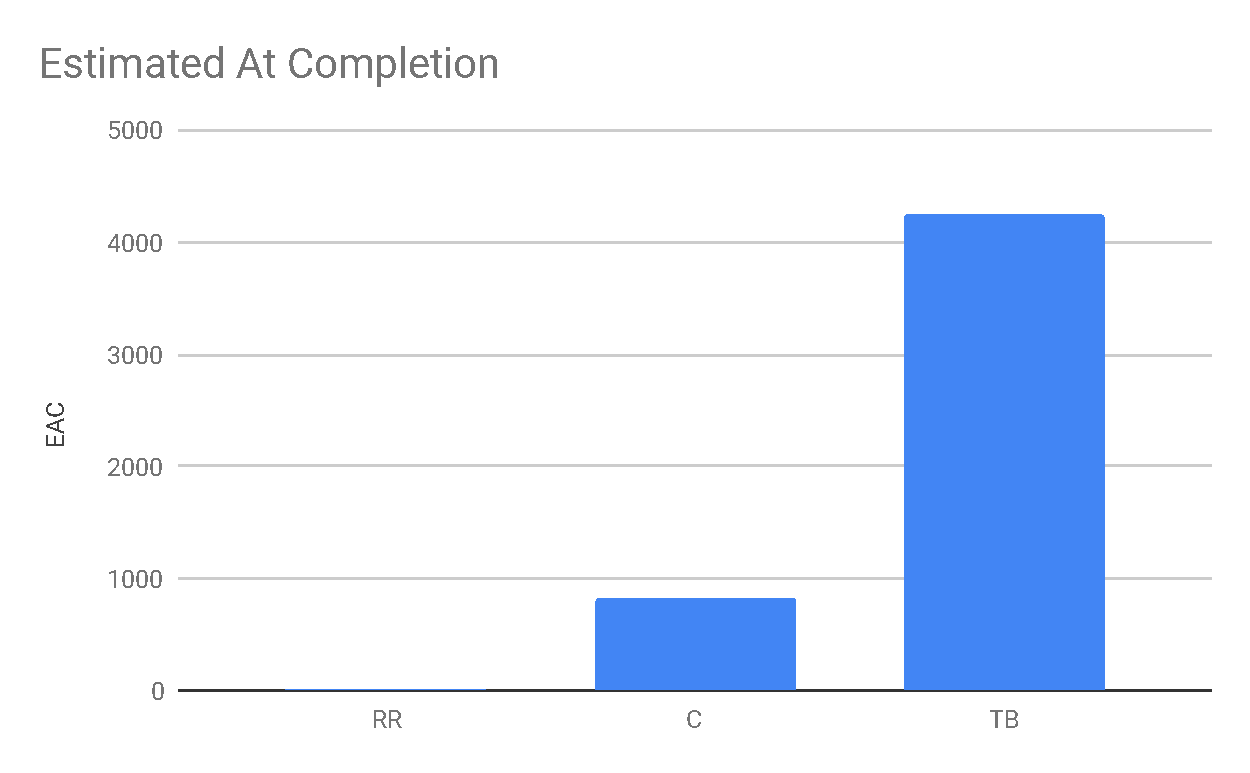
\includegraphics[scale=0.7]{res/images/RA/eac.pdf}
	\caption{Andamento dell'Estimated At Completion durante il progetto}
\end{figure}
\paragraph*{Valutazione}

Le differenze nelle spese sostenute (-144\euro in TB, +355\euro in PB) non sono state tanto gravi da inficiare il preventivo a finire, ragion per cui EAC rimane invariato e di valore pari al preventivo.\\
La soglia prevista del 5\% è pienamente rispettata.

%\subsubsection{Profondità della gerarchia}

\subsubsection{VAC - Variance At Completion}
\begin{figure}[H]
	\centering
	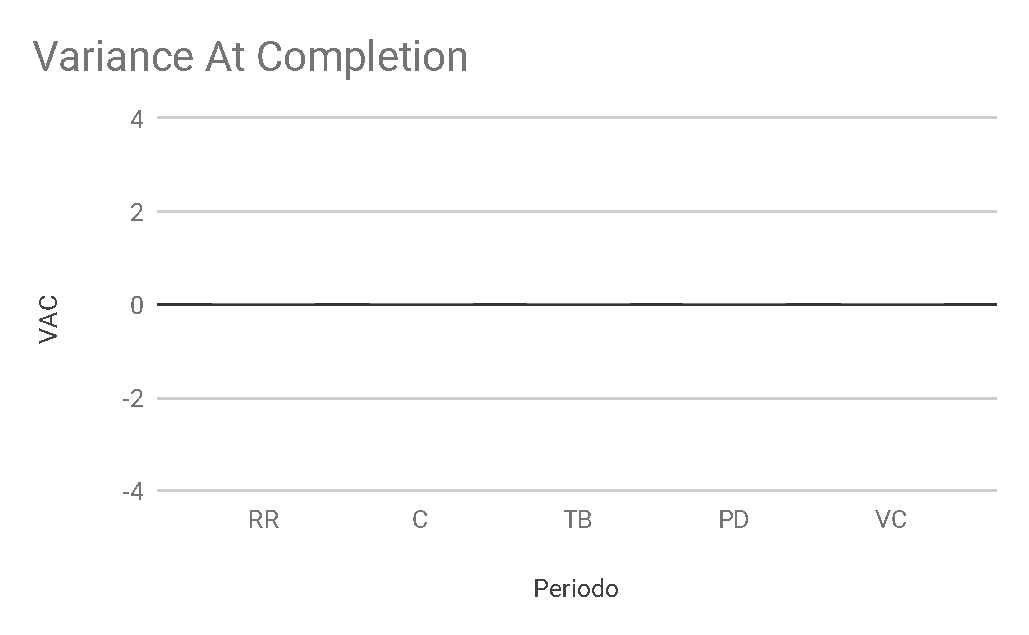
\includegraphics[scale=0.7]{res/images/RA/vac.pdf}
	\caption{Andamento della Variance At Completion durante il progetto}
\end{figure}
\paragraph*{Valutazione}
La differenza tra preventivo e EAC rimane invariata nei periodi e pari a zero; dunque VAC, cioè la percentuale della differenza, è ugualmente invariata e pari a zero. \\
L'obiettivo di avere $VAC \geq 0\%$ è raggiunto.

\subsubsection{EV - Earned Value}
\begin{figure}[H]
	\centering
	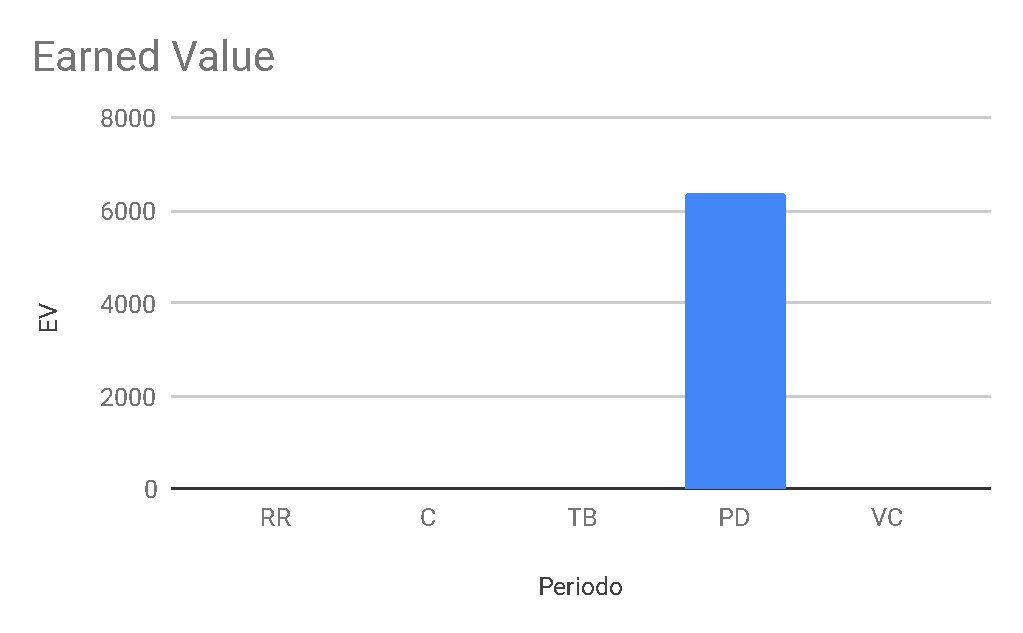
\includegraphics[scale=0.7]{res/images/RA/ev.pdf}
	\caption{Andamento dell'Earned Value durante il progetto}
\end{figure}
\paragraph*{Valutazione}
Possiamo notare che, nonostante il lavoro svolto non ci sia stato alcun guadagno prima della PB. L'EV dipende dalla quantità di obiettivi raggiunti, misurata dal numero di requisiti soddisfatti: ecco spiegata la tardiva produzione di valore.\\
Durante la PB sarebbe stato preferibile aver soddisfatto dimostrabilmente un numero maggiore di requisiti: in mancanza di ciò, in RA avremo un carico di lavoro maggiore rispetto alle attività previste. 

\subsubsection{AC - Actual Cost}
\begin{figure}[H]
	\centering
	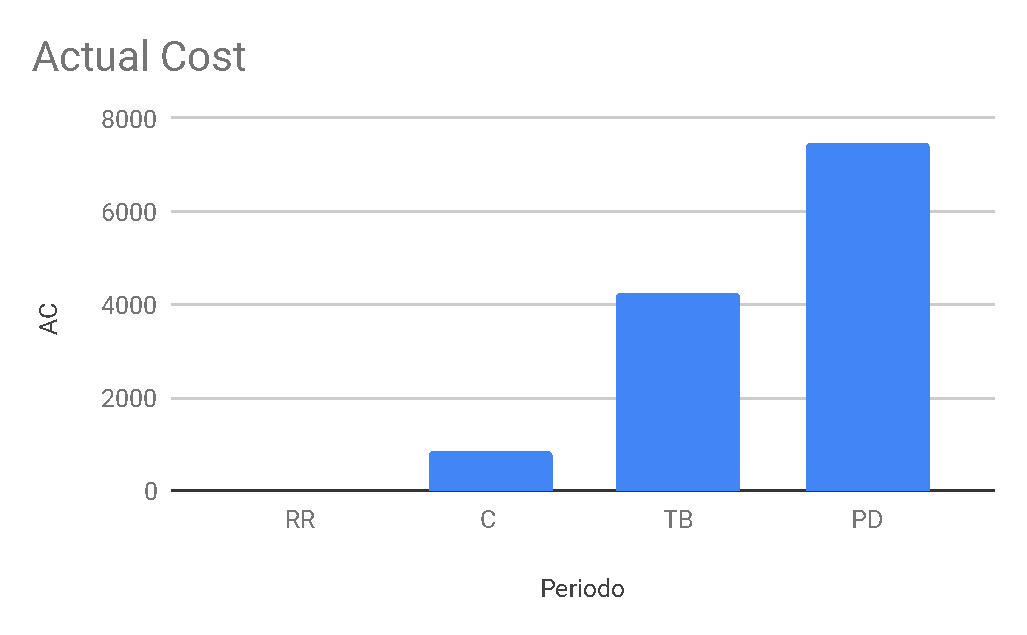
\includegraphics[scale=0.7]{res/images/RA/ac.pdf}
	\caption{Andamento dell'Actual Cost durante il progetto}
\end{figure}
\paragraph*{Valutazione}
Il costo effettivo del lavoro, durante ogni fase, non si è molto discostato da quanto preventivato: dunque la pianificazione svolta risulta adeguata rispetto ai costi del lavoro previsti. \\
Durante la fase di PB, AC ha superato PV, dunque la soglia di ottimalità $0 \leq AC < PV$ è stata infranta. La soglia di accettabilità invece è sempre stata rispettata.

\subsubsection{PV - Planned Value}
% IPOTESI: 20% dei req soddisfatti in TB, 80% in PB, 100% in VC
\begin{figure}[H]
	\centering
	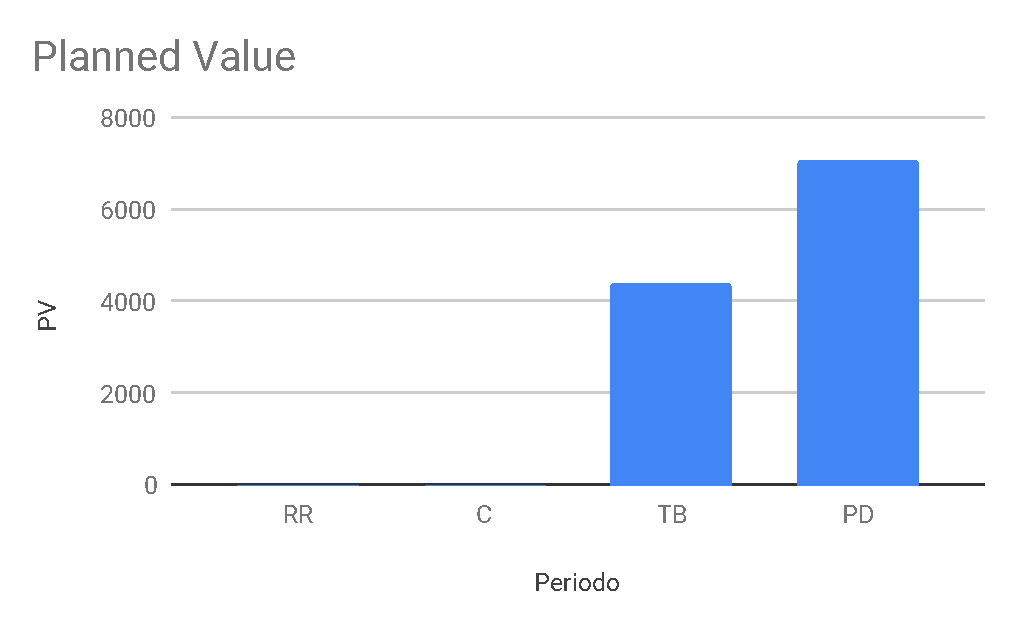
\includegraphics[scale=0.7]{res/images/RA/pv.pdf}
	\caption{Andamento del Planned Value durante il progetto}
\end{figure}
\paragraph*{Valutazione}
Il PV riporta semplicemente il valore del lavoro preventivato fino al momento del calcolo.

\subsubsection{SV - Schedule Variance}
\begin{figure}[H]
	\centering
	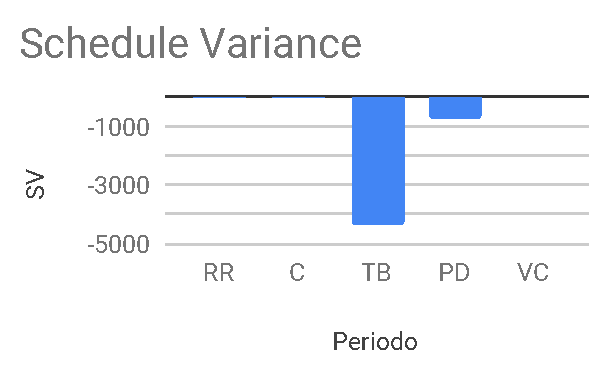
\includegraphics[scale=0.7]{res/images/RA/sv.pdf}
	\caption{Andamento della Schedule Variance durante il progetto}
\end{figure}
\paragraph*{Valutazione}
Durante il periodo di TB il valore è preoccupante: il fatto è che non è stato considerato completato alcun requisito, mentre molte spese erano previste.\\
Durante il periodo di PB sono stati soddisfatti molti requisiti, quindi EV è cresciuto, ma non a sufficienza da coprire le spese previste.\\
Le soglie imposte per la metrica appaiono troppo restrittive, quindi inadeguate rispetto alla pianificazione del progetto.

\subsubsection{CV - Cost Variance}
\begin{figure}[H]
	\centering
	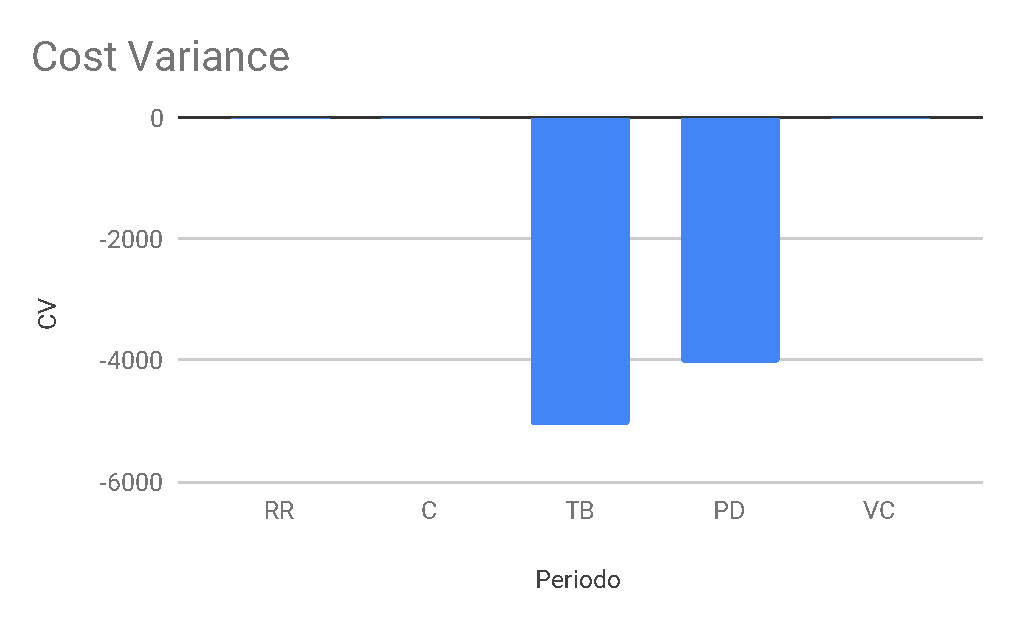
\includegraphics[scale=0.7]{res/images/RA/cv.pdf}
	\caption{Andamento della Cost Variance durante il progetto}
\end{figure}
\paragraph*{Valutazione}
Valgono i ragionamenti fatti in SV per quanto riguarda EV.

%\pagebreak
\subsubsection{Code Coverage}
\paragraph{Statement coverage}\mbox{}\\
\begin{figure}[H]
	\centering
	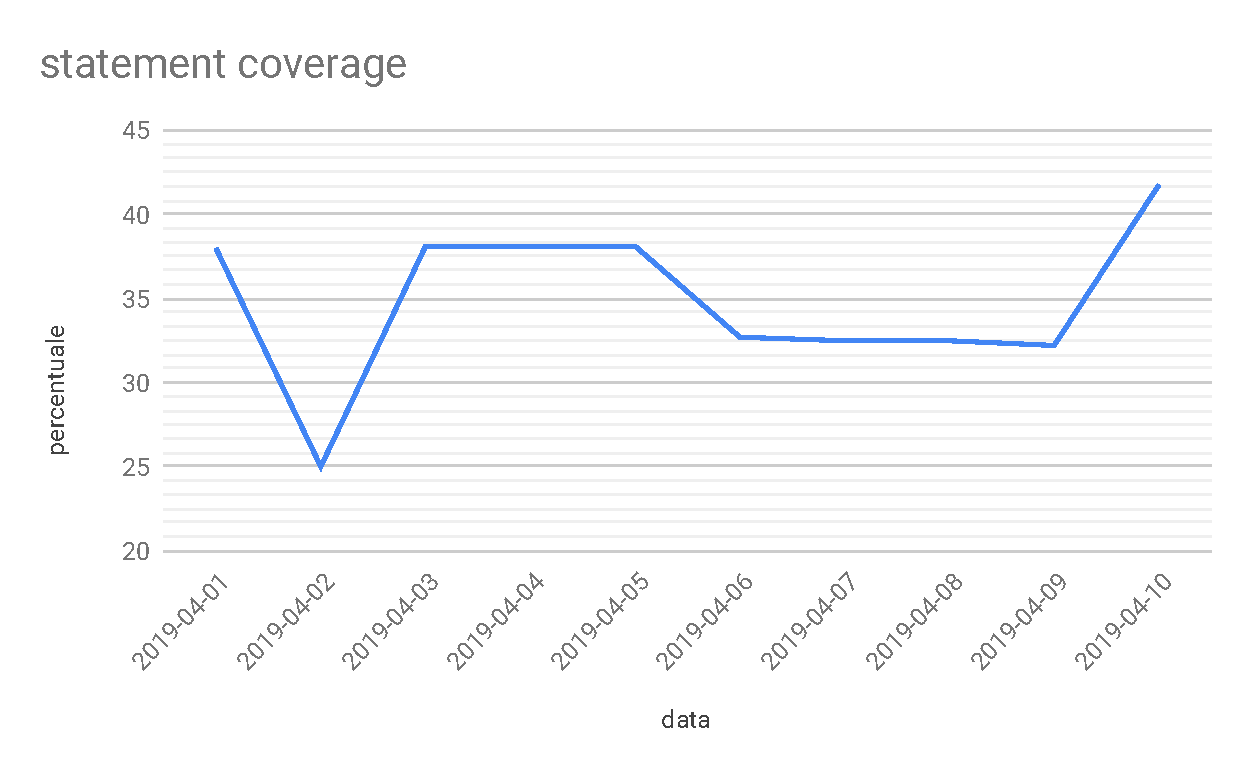
\includegraphics[scale=0.6]{res/images/RA/statement-coverage-RQ.pdf}
	\caption{Statement coverage}
\end{figure}	
\paragraph{Branch coverage}\mbox{}\\
\begin{figure}[H]
	\centering
	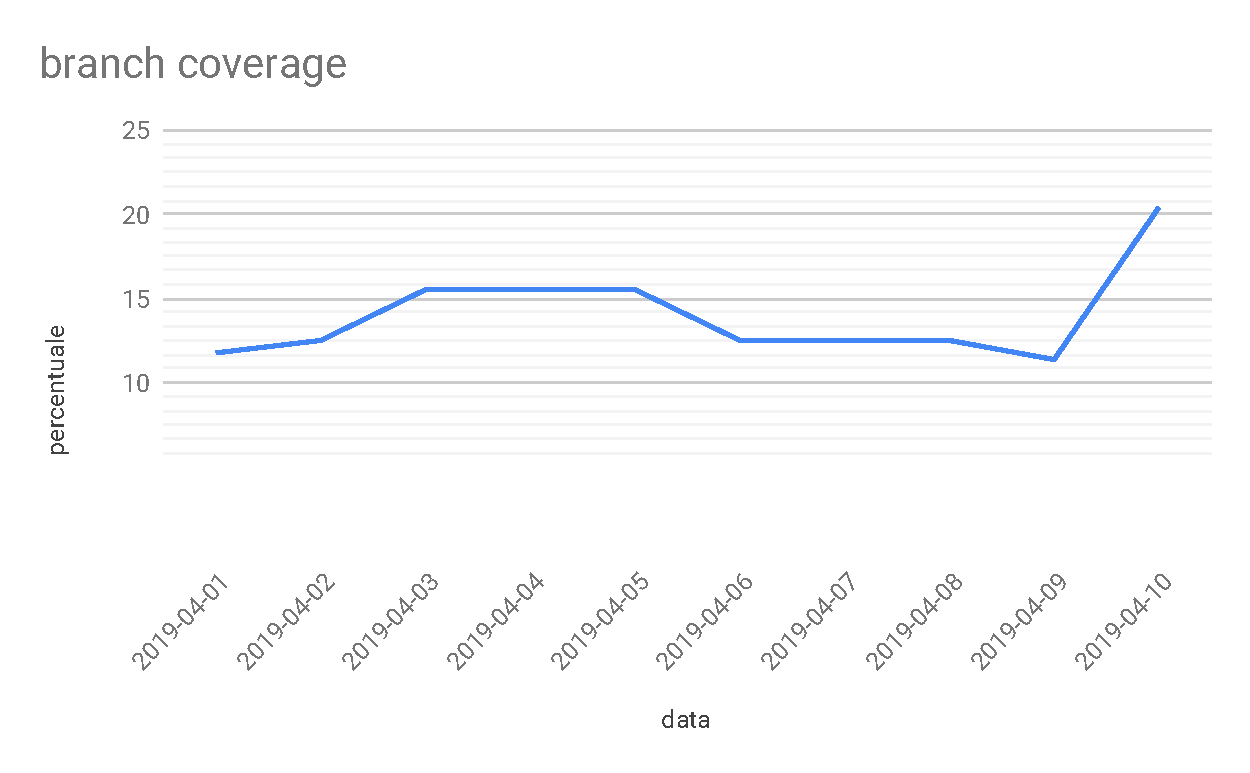
\includegraphics[scale=0.6]{res/images/RA/branch-coverage-RQ.pdf}
	\caption{Branch coverage}
\end{figure}
\paragraph{Function coverage}\mbox{}\\
\begin{figure}[H]
	\centering
	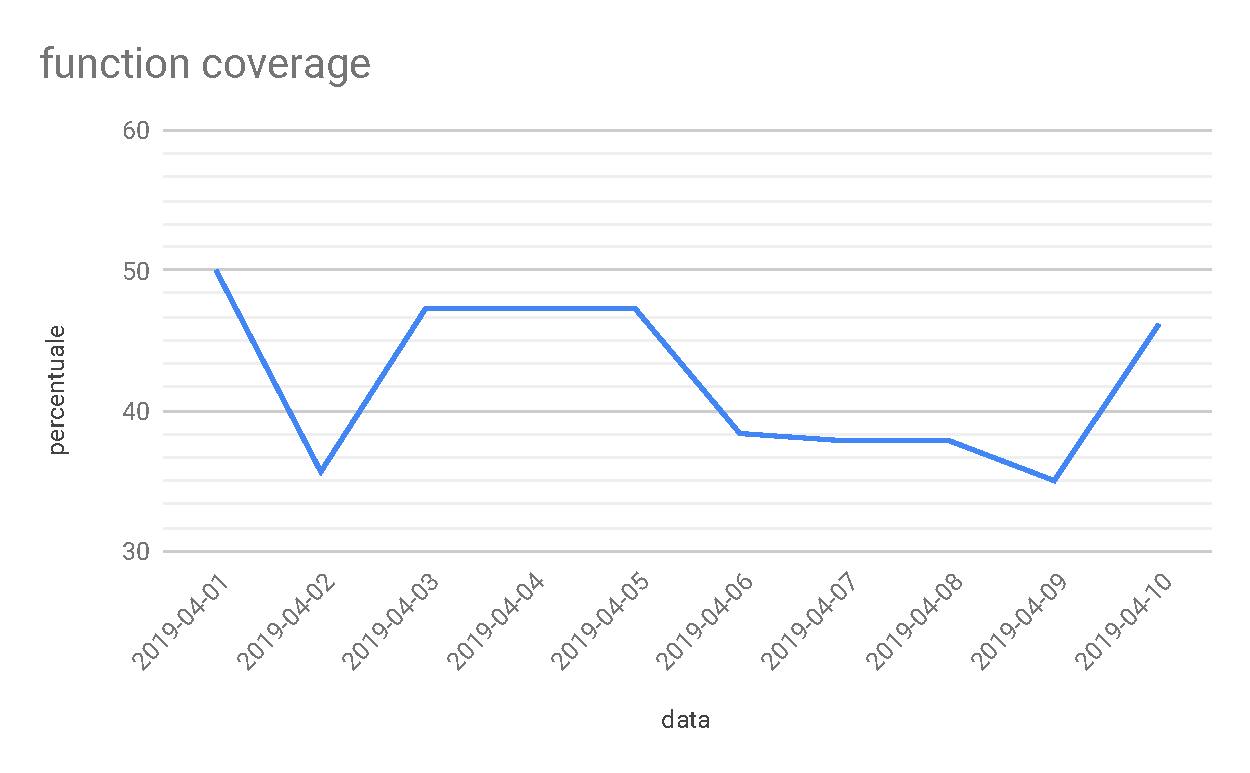
\includegraphics[scale=0.6]{res/images/RA/function-coverage-RQ.pdf}
	\caption{Function coverage}
\end{figure}
\paragraph{Line coverage}\mbox{}\\
\begin{figure}[H]
	\centering
	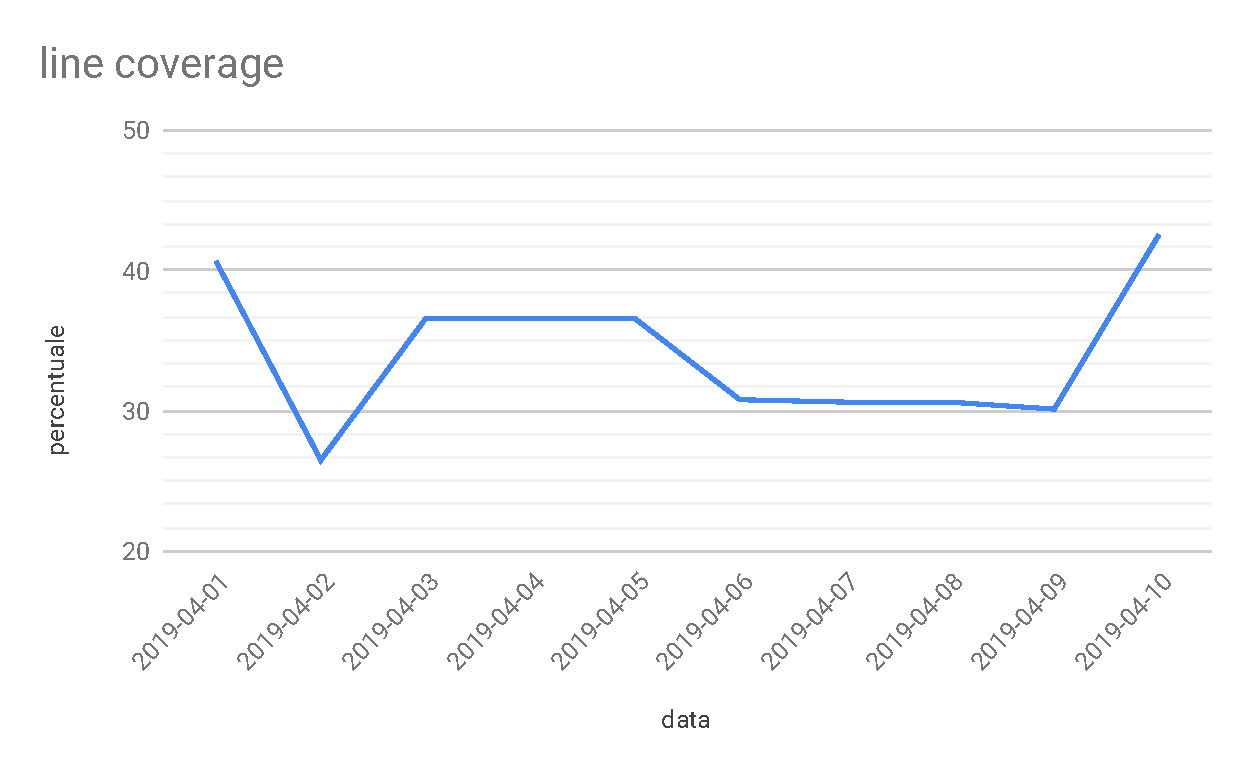
\includegraphics[scale=0.6]{res/images/RA/line-coverage-RQ.pdf}
	\caption{Line coverage}
\end{figure}
\paragraph*{Valutazione complessiva}
Complessivamente la metrica del coverage ha un'andamento prevedibile e si avvicina alle soglie desiderate.
La metrica è stata messa in opera mentre codice e test venivano implementati parallelamente: ecco perché nel periodo iniziale l'andamento del coverage è altalenante.
L'aumento della copertura, a partire dal 10 aprile, corrisponde a una progressione nei test mentre l'ampiezza della codebase rimaneva invariata.
%\subsubsection{Facilità di utilizzo}

\subsection{Facilità di utilizzo}
\begin{figure}[H]
	\centering
	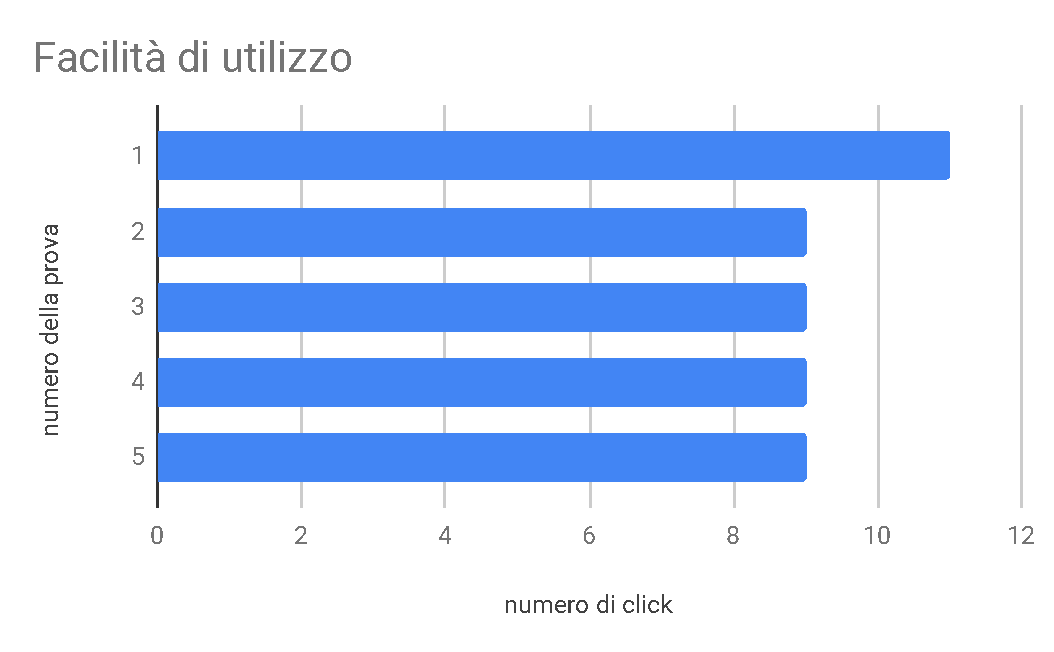
\includegraphics[scale=0.6]{res/images/RA/facilita-di-utilizzo.pdf}
	\caption{Facilità di utilizzo}
\end{figure}
\paragraph*{Valutazione}
Il numero di click è sufficientemente basso, considerando che il loro conteggio parte dalla registrazione.
La metrica rispetta la soglia preferibile desiderata di 10 click.
 
\subsection{Facilità di apprendimento}
\begin{figure}[H]
	\centering
	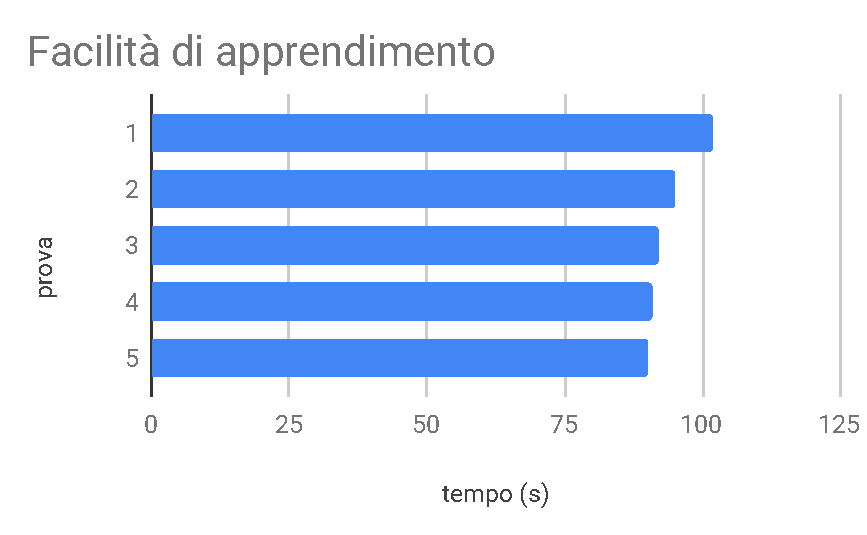
\includegraphics[scale=0.7]{res/images/RA/facilita-di-apprendimento.pdf}
	\caption{Facilità di apprendimento}
\end{figure}
\paragraph*{Valutazione}
Anche in questo caso il conteggio comincia dalla registrazione. Il tempo richiesto a completare l'acquisto supera ampiamente la soglia preferibile di 3 minuti di tempo. 

\subsubsection{Facilità di comprensione} % == CCR
\begin{figure}[H]
	\centering
	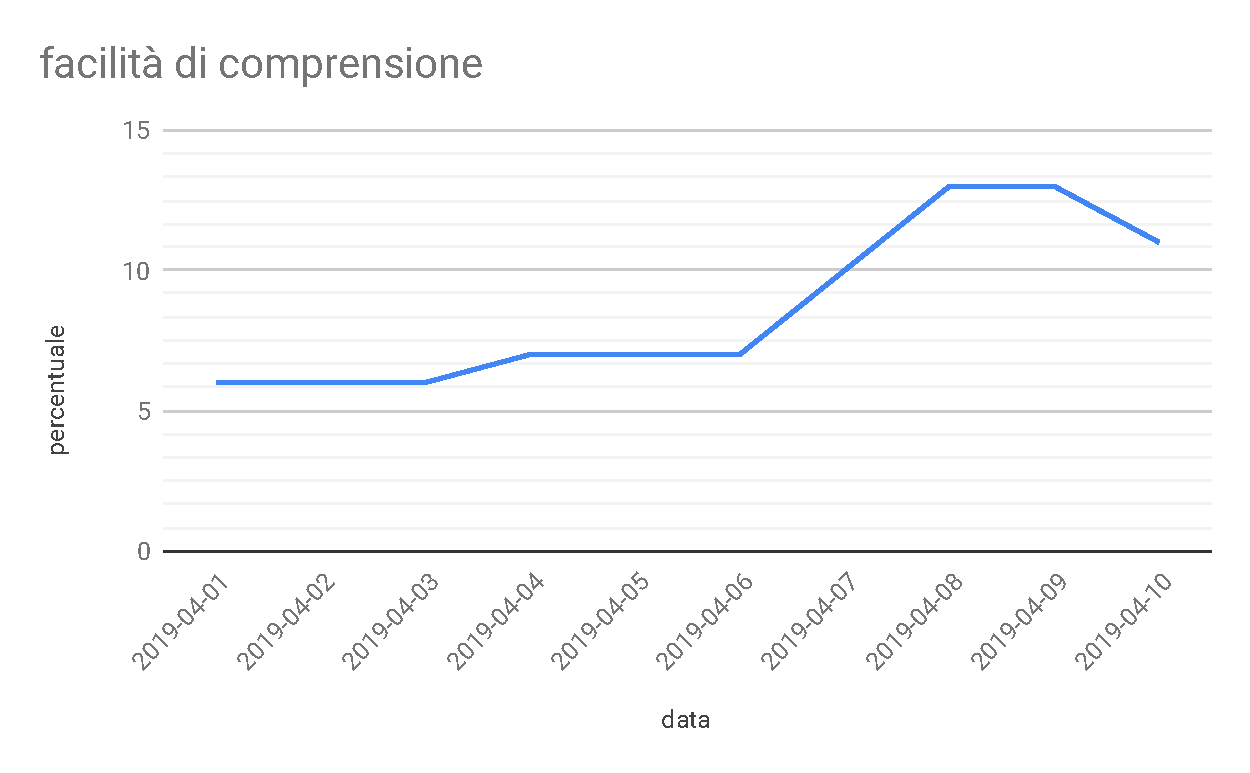
\includegraphics[scale=0.6]{res/images/RA/facilita-di-comprensione.pdf}
	\caption{Facilità di comprensione}
\end{figure}
\paragraph*{Valutazione}
La quantità di commenti rispetto al codice, inizialmente bassa e sregolata, tende alla soglia di accettabilità del 10\% per volere del gruppo di avere un codice chiaro e comprensibile. 

\pagebreak
\subsubsection{Indice di Gulpease}

\begin{longtable}{ >{\centering}p{0.15\textwidth} >{\centering}p{0.10\textwidth}	>{\centering}p{0.1075\textwidth} >{\centering}p{0.10\textwidth} >{\centering}p{0.10\textwidth} >{\centering}p{0.10\textwidth}}
	
	%\hline
	\rowcolor{white}\caption{Indice di Gulpease raggruppato per documento, lungo i periodi da RR a TB}\\
	\rowcolorhead
	\textbf{\color{white}N} 
	& \textbf{\color{white}RR} 
	& \centering\textbf{\color{white}C}
	& \textbf{\color{white}TB}
	& \textbf{\color{white}PD}
	& \textbf{\color{white}VC} 
	\tabularnewline %\hline 	
	
	\textit{Analisi dei requisiti}
	& 67
	& 66
	& 63
	& 63
	& -
	\tabularnewline %\hline 
	
	\textit{Glossario}
	& 71
	& 71
	& 71
	& 71
	& -
	\tabularnewline %\hline 
	
	\textit{Norme di progetto}
	& 65
	& 65
	& 63
	& 66
	& -
	\tabularnewline %\hline 
	
	\textit{Piano di progetto}
	& 68
	& 68
	& 66
	& 67
	& -
	\tabularnewline %\hline 
	
	\textit{Piano di qualifica}
	& 70
	& 70
	& 67
	& 65
	& -
	\tabularnewline %\hline 
	
	\textit{Studio di Fattibilità}
	& 73
	& -
	& -
	& -
	& -
	\tabularnewline %\hline 
	
	\textit{Verbali esterni (media)}
	& 72
	& 72
	& 66
	& 69
	& -
	\tabularnewline %\hline 
	
	\textit{Verbali interni (media)}
	& 74
	& 74
	& 70
	& 73
	& -
\end{longtable}
\begin{figure}[H]
	\centering
	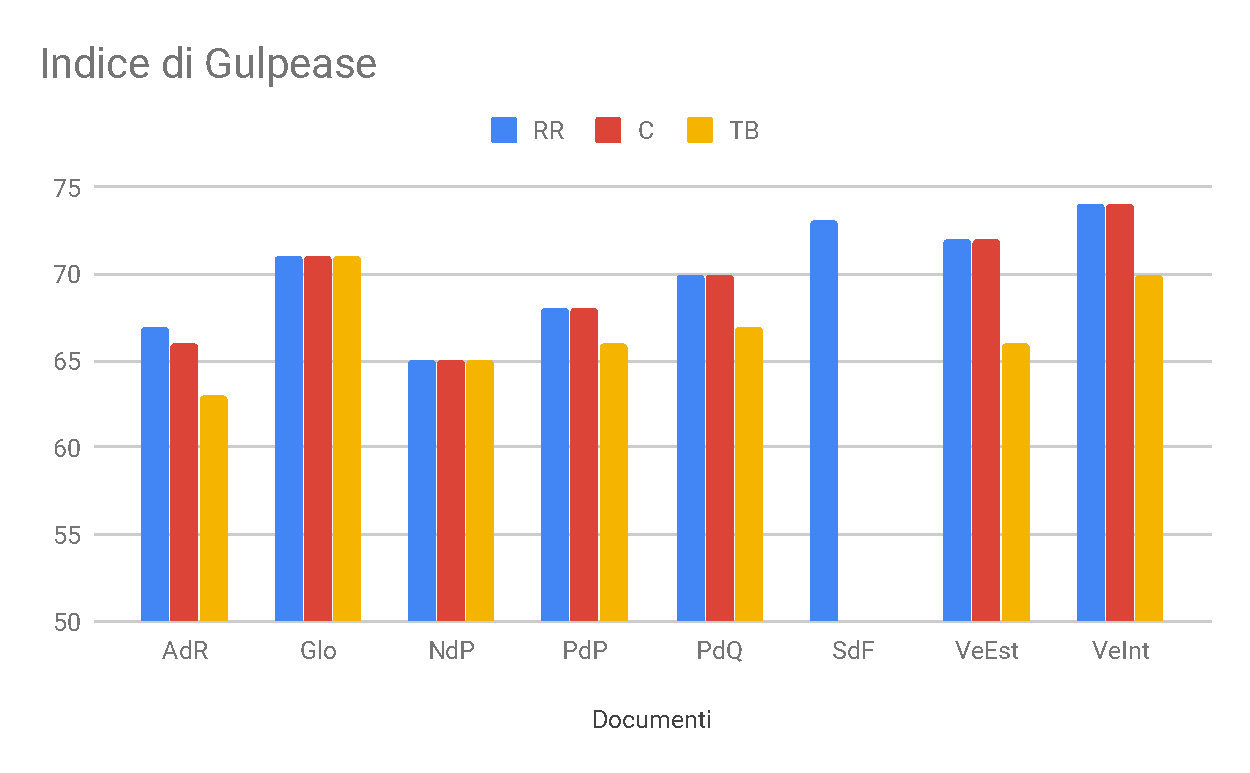
\includegraphics[scale=0.8]{res/images/RA/gulpease.pdf}
	\caption{Indice di Gulpease}
\end{figure}

\paragraph*{Valutazione}
Fino alla fase C l'indice è stato calcolato con uno strumento diverso rispetto alle fasi successive: questo spiega la discordanza tra i valori prima e dopo.
In generale, nonostante l'impegno del gruppo nella semplificazione della sintassi, l'indice non sembra migliorare molto.
Questo può indicare una generale difficoltà nel semplificare documenti di natura tecnica.\\
A una valutazione posteriore, la soglia di ottimalità imposta appare eccessivamente ottimistica: un valore $>80$ infatti indica un testo leggibile con facilità da bambini delle elementari.\\
La soglia di accettabilità invece sono plausibili e rispettate. 

%\subsubsection{Semplicità delle classi}

\subsubsection{SLOC}
\begin{figure}[H]
	\centering
	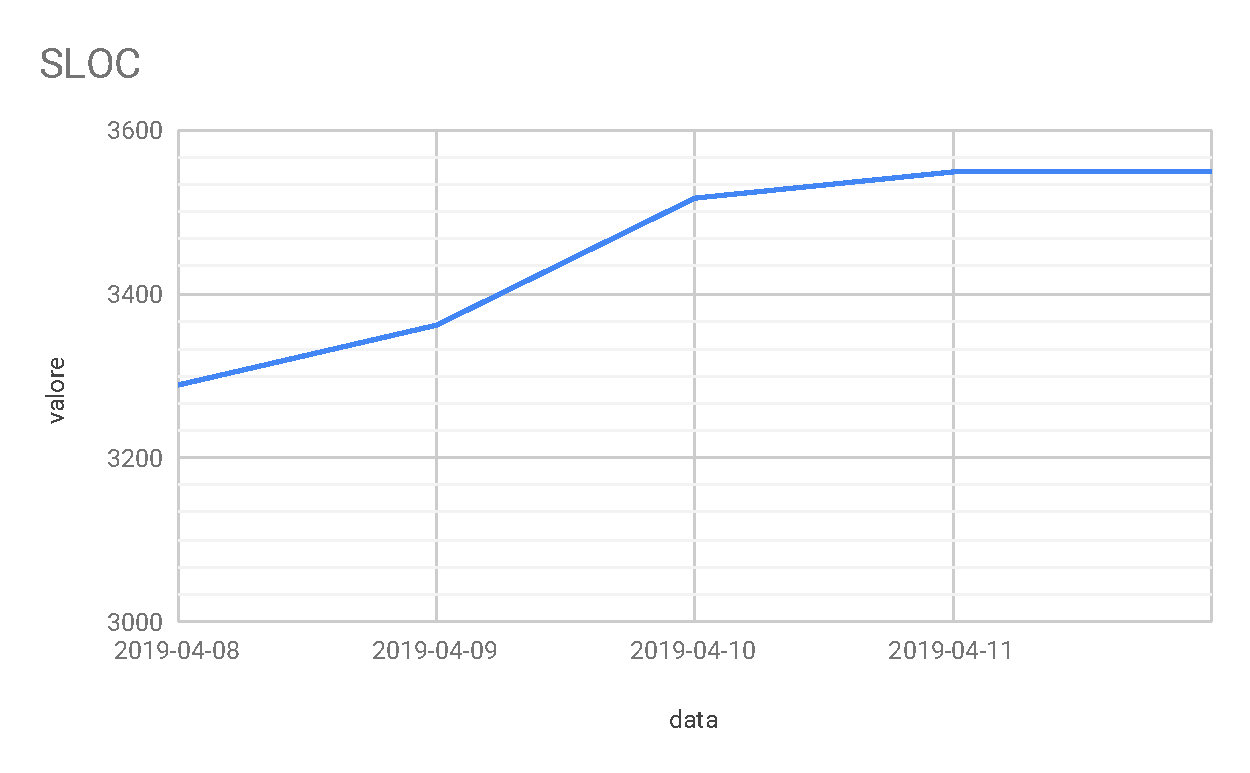
\includegraphics[scale=0.6]{res/images/RA/sloc.pdf}
	\caption{Source lines of code}
\end{figure}
\paragraph*{Valutazione}
Lo SLOC ha un'andamento prevedibile tendente al logaritmo, che indica una stabilità delle righe totali di codice del prodotto man mano che il progetto si avvicina alla fine. Le soglie di accettabilità e ottimalità sono rispettate.




\pagebreak
\section{Valutazioni per il miglioramento}


%\pagebreak
%\section{Tracciamento}  
 % (probabilmente) da fare dopo l'RR


\end{document}
